\newcommand{\VL}{$V_{L}$~}
\newcommand{\csTh}{$\cos \theta^{*}$~}

\section{Partial width of top-quark decay}

The partial width of the top-quark decay can be expressed in terms of the anomalous couplings in the $Wtb$ interaction as represented in the following equations.\\
The first and less extensive one describes the longitudinal decay.

\begin{eqnarray}
  \Gamma_{0} & = & \frac{g^{2} \vert \vec{q}}{32 \pi} \left\lbrace \frac{m_{t}^{2}}{m_{W}^{2}} \left[ \vert V_{L} \vert^{2} + \vert V_{R} \vert^{2} \right] (1 - x_{W}^{2} - 2x_{b}^{2} -x_{W}^{2} x_{b}^{2} + x_{b}^{4}) - 4x_{b}Re V_{L}V_{R}^{*} \right. \nonumber \\
             &   & + \left[ \vert g_{L} \vert^{2} + \vert g_{R} \vert^{2} \right] (1 - x_{W}^{2} + x_{b}^{2}) - 4 x_{b} Re g_{L} g_{R}^{*} \nonumber \\
             &   & - 2 \frac{m_{t}}{m_{W}} Re \left[ V_{L}g_{R}^{*} + V_{R}g_{L}^{*} \right] (1- x_{W}^{2} - x_{b}^{2}) \nonumber \\
             &   & \left. +2 \frac{m_t}{m_W} x_b Re \left[ V_{L}g_{L}^{*} + V_{R}g_{R}^{*} \right] (1+ x_{W}^{2} - x_{b}^{2}) \right\rbrace
\end{eqnarray}

with:
\begin{subequations} \label{eq::Simplified}
 \begin{align} 
  x_W & = \frac{m_{W}}{m_{t}} \\
  x_b & = \frac{m_{b}}{m_{t}} \\
  \vert \vec{q} \vert & = \frac{1}{2 m_{t}} \sqrt{m_{t}^{4} + m_{W}^{4} + m_{b}^{4} - 2m_{t}^{2} m_{W}^{2} - 2m_{t}^{2} m_{b}^{2} - 2m_{W}^{2}m_{b}^{2}}  
 \end{align}
\end{subequations}

A similar equation can also be formulated for the left- and right-handed top-quark decay, which only differ partially with a minus sign. The right-handed part corresponds to the plus-sign option while the left-handed contribution contains the minus-sign.
\begin{eqnarray}
 \Gamma_{R,L} & = & \frac{g^{2} \vert \vec{q}}{32 \pi} \left\lbrace \frac{m_{t}^{2}}{m_{W}^{2}} \left[ \vert V_{L} \vert^{2} + \vert V_{R} \vert^{2} \right] (1 - x_{W}^{2} + x_{b}^{2}) - 4x_{b}Re V_{L}V_{R}^{*} \right. \nonumber \\
            &   & + \frac{m_{t}^{2}}{m_{W}^{2}} \left[ \vert g_{L} \vert^{2} + \vert g_{R} \vert^{2} \right] (1 - x_{W}^{2} - 2x_{b}^{2} -x_{W}^{2} x_{b}^{2} + x_{b}^{4}) - 4x_{b}Re g_{L}g_{R}^{*} \nonumber \\
            &   & - 2 \frac{m_t}{m_W} Re \left[ V_{L}g_{R}^{*} + V_{R}g_{L}^{*} \right] (1- x_{W}^{2} - x_{b}^{2}) \nonumber \\
            &   &  \left. + 2 \frac{m_t}{m_W} x_b Re \left[ V_{L}g_{L}^{*} + V_{R}g_{R}^{*} \right] (1+ x_{W}^{2} - x_{b}^{2}) \right\rbrace \nonumber \\
           &   & \pm \frac{g^{2}}{64 \pi} \frac{m_{t}^{3}}{m_{W}^{2}} \left\lbrace -x_{W}^{2} \left[ \vert V_{L} \vert^{2} - \vert V_{R} \vert^{2} + \vert g_{L} \vert^{2} - \vert g_{R} \vert^{2} \right] (1-x_{b}^{2}) \right. \nonumber \\
            &   &  \left. + 2 x_{W} Re \left[ V_{L}g_{R}^{*} + V_{R}g_{L}^{*} \right] + 2x_{W} x_{b} Re \left[ V_{L}g_{L}^{*} + V_{R}g_{R}^{*} \right] \right\rbrace \nonumber \\
            &   & \times (1-2x_{W}^{2} - 2x_{b}^{2} + x_{W}^{4} - 2x_{W}^{2} x_{b}^{2} + x_{b}^{4})
\end{eqnarray}

In order to transform these partial width formulas into helicity fractions, also the total width of the top quark decay is needed. This because each helicity fraction is defined as the corresponding partial width divided by the total width.

\begin{eqnarray}
 \Gamma & = & \frac{g^{2} \vert \vec{q}}{32 \pi} \frac{m_{t}^{2}}{m_{W}^{2}} \left\lbrace \left[ \vert V_{L} \vert^{2} + \vert V_{R} \vert^{2} \right] (1 + x_{W}^{2} - 2x_{b}^{2} - 2 x_{W}^{4} + x_{W}^{2} x_{b}^{2} + x_{b}^{4}) - 4x_{b}Re V_{L}V_{R}^{*} \right. \nonumber \\
        &   & -12 x_{W}^{2} x_{b} Re V_{L} V_{R}^{*} + 2 \left[ \vert g_{L} \vert^{2} + \vert g_{R} \vert^{2} \right] \left( 1 - \frac{x_{W}^{2}}{2} - 2 x_{b}^{2} - \frac{x_{X}^{4}}{2} - \frac{x_{W}^{2} x_{b}^{2}}{2} +x_{b}^{4} \right) \nonumber \\
        &   & -12 x_{W}^{2} x_{b} Re g_{L} g_{R}^{*} - 6 x_{W} Re \left[ V_{L}g_{R}^{*} + V_{R}g_{L}^{*} \right] (1 - x_{W}^{2} - x_{b}^{2}) \nonumber \\
        &   & \left. 6 x_{W} x_{b} Re \left[ V_{L}g_{L}^{*} + V_{R}g_{R}^{*} \right] (1 + x_{W}^{2} - x_{b}^{2}) \right\rbrace
\end{eqnarray}

\section{Simplification in limit-cases}
\subsection{Only 1 coupling non-zero}
If we consider the case where only the \VL coupling parameter is non-zero, the above definitions get reduced to the following formulas.

\begin{eqnarray}
 \Gamma_{0} & = & \frac{g^{2} \vert \vec{q}}{32 \pi} \frac{m_{t}^{2}}{m_{W}^{2}} \vert V_{L} \vert^{2} (1 - x_{W}^{2} - 2x_{b}^{2} -x_{W}^{2} x_{b}^{2} + x_{b}^{4}) \\
 \Gamma_{R,L} & = & \frac{g^{2} \vert \vec{q}}{32 \pi}  \vert V_{L} \vert^{2} (1 - x_{W}^{2} + x_{b}^{2}) \pm \frac{g^{2}}{64 \pi} \frac{m_{t}^{3}}{m_{W}^{2}} \left\lbrace -x_{W}^{2}  \vert V_{L} \vert^{2} (1-x_{b}^{2}) \right\rbrace \\
 \Gamma & = & \frac{g^{2} \vert \vec{q}}{32 \pi} \frac{m_{t}^{2}}{m_{W}^{2}} \vert V_{L} \vert^{2} (1 + x_{W}^{2} - 2x_{b}^{2} - 2 x_{W}^{4} + x_{W}^{2} x_{b}^{2})
\end{eqnarray}

So this implies that the helicity fractions can be defined as follows:

\begin{eqnarray}
 F_{0}   & = \frac{\Gamma_{0}}{\Gamma} =   & \frac{(1 - x_{W}^{2} - 2x_{b}^{2} -x_{W}^{2} x_{b}^{2} + x_{b}^{4})}{(1 + x_{W}^{2} - 2x_{b}^{2} - 2 x_{W}^{4} + x_{W}^{2} x_{b}^{2})} \label{eq::F0MasslessB} \\
 F_{R,L} & = \frac{\Gamma_{R,L}}{\Gamma} = & \frac{m_{W}^{2}}{m_{t}^{2}} \frac{(1 - x_{W}^{2} + x_{b}^{2})}{(1 + x_{W}^{2} - 2x_{b}^{2} - 2 x_{W}^{4} + x_{W}^{2} x_{b}^{2})} \nonumber \\
         &                                 & \pm \frac{m_{t}}{2 \vert \vec{q} \vert} \frac{ -x_{W}^{2} (1-x_{b}^{2})}{(1 + x_{W}^{2} - 2x_{b}^{2} - 2 x_{W}^{4} + x_{W}^{2} x_{b}^{2})} \label{eq::FRLMasslessB}
\end{eqnarray}

From the above two equations can easily be concluded that in cases where only one of the Wtb-coupling coefficients is non-zero, there will be no influence visible on the helicity fractions. This because no interference between different coupling coefficients occurs which allows the cancellation of this single coupling coefficient. This behavior is indeed retrieved in the different \csTh distributions which have been studied in detail. The ones with only one coupling constant active can be found in Figure \ref{fig::CosThetaOneCoupling}.\\

\begin{figure}[h!]
 \centering
 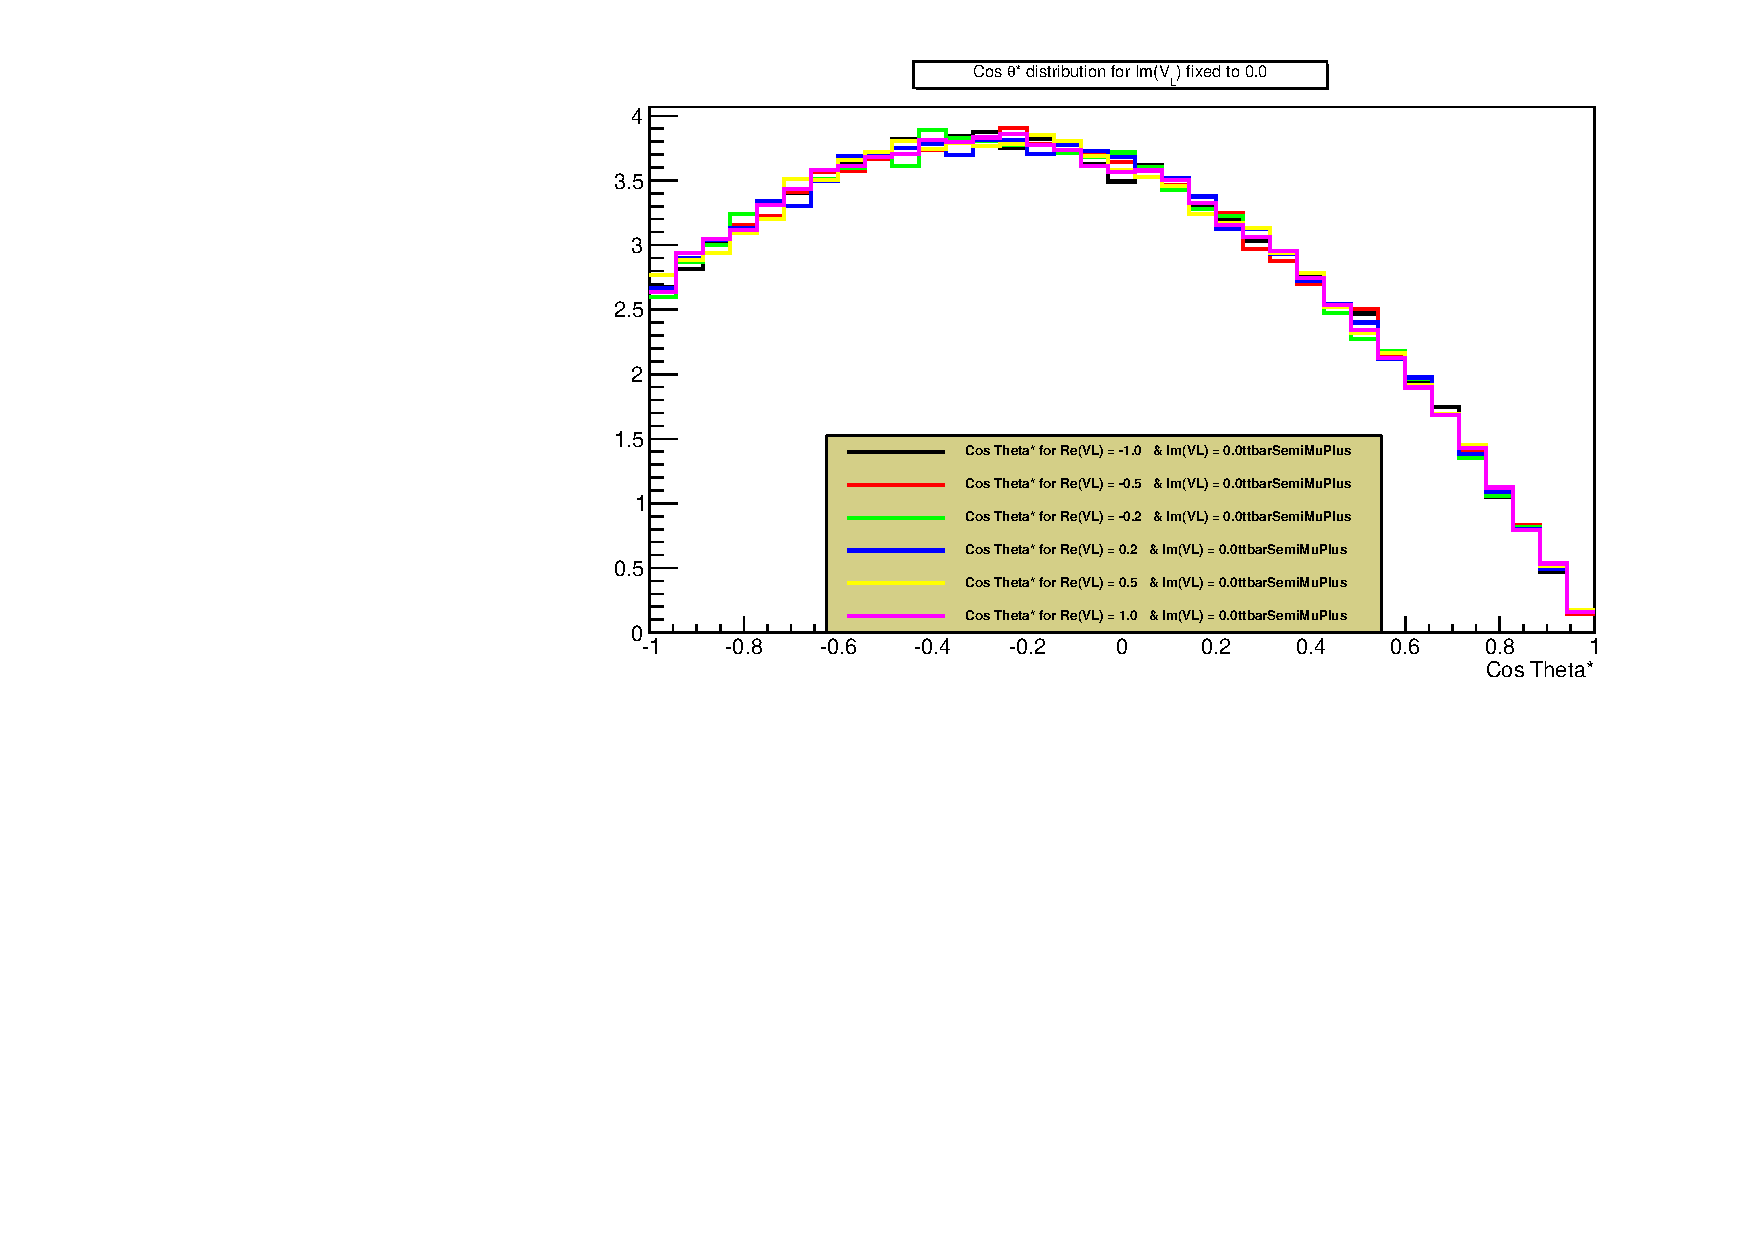
\includegraphics[width = 0.45 \textwidth]{Afbeeldingen/Chapter_LinkWithTopWidth/CosThetaResults/RVLvsIVL/RVLIVL_CosTheta_IVLFixedTo00.pdf}    %RVL varied
 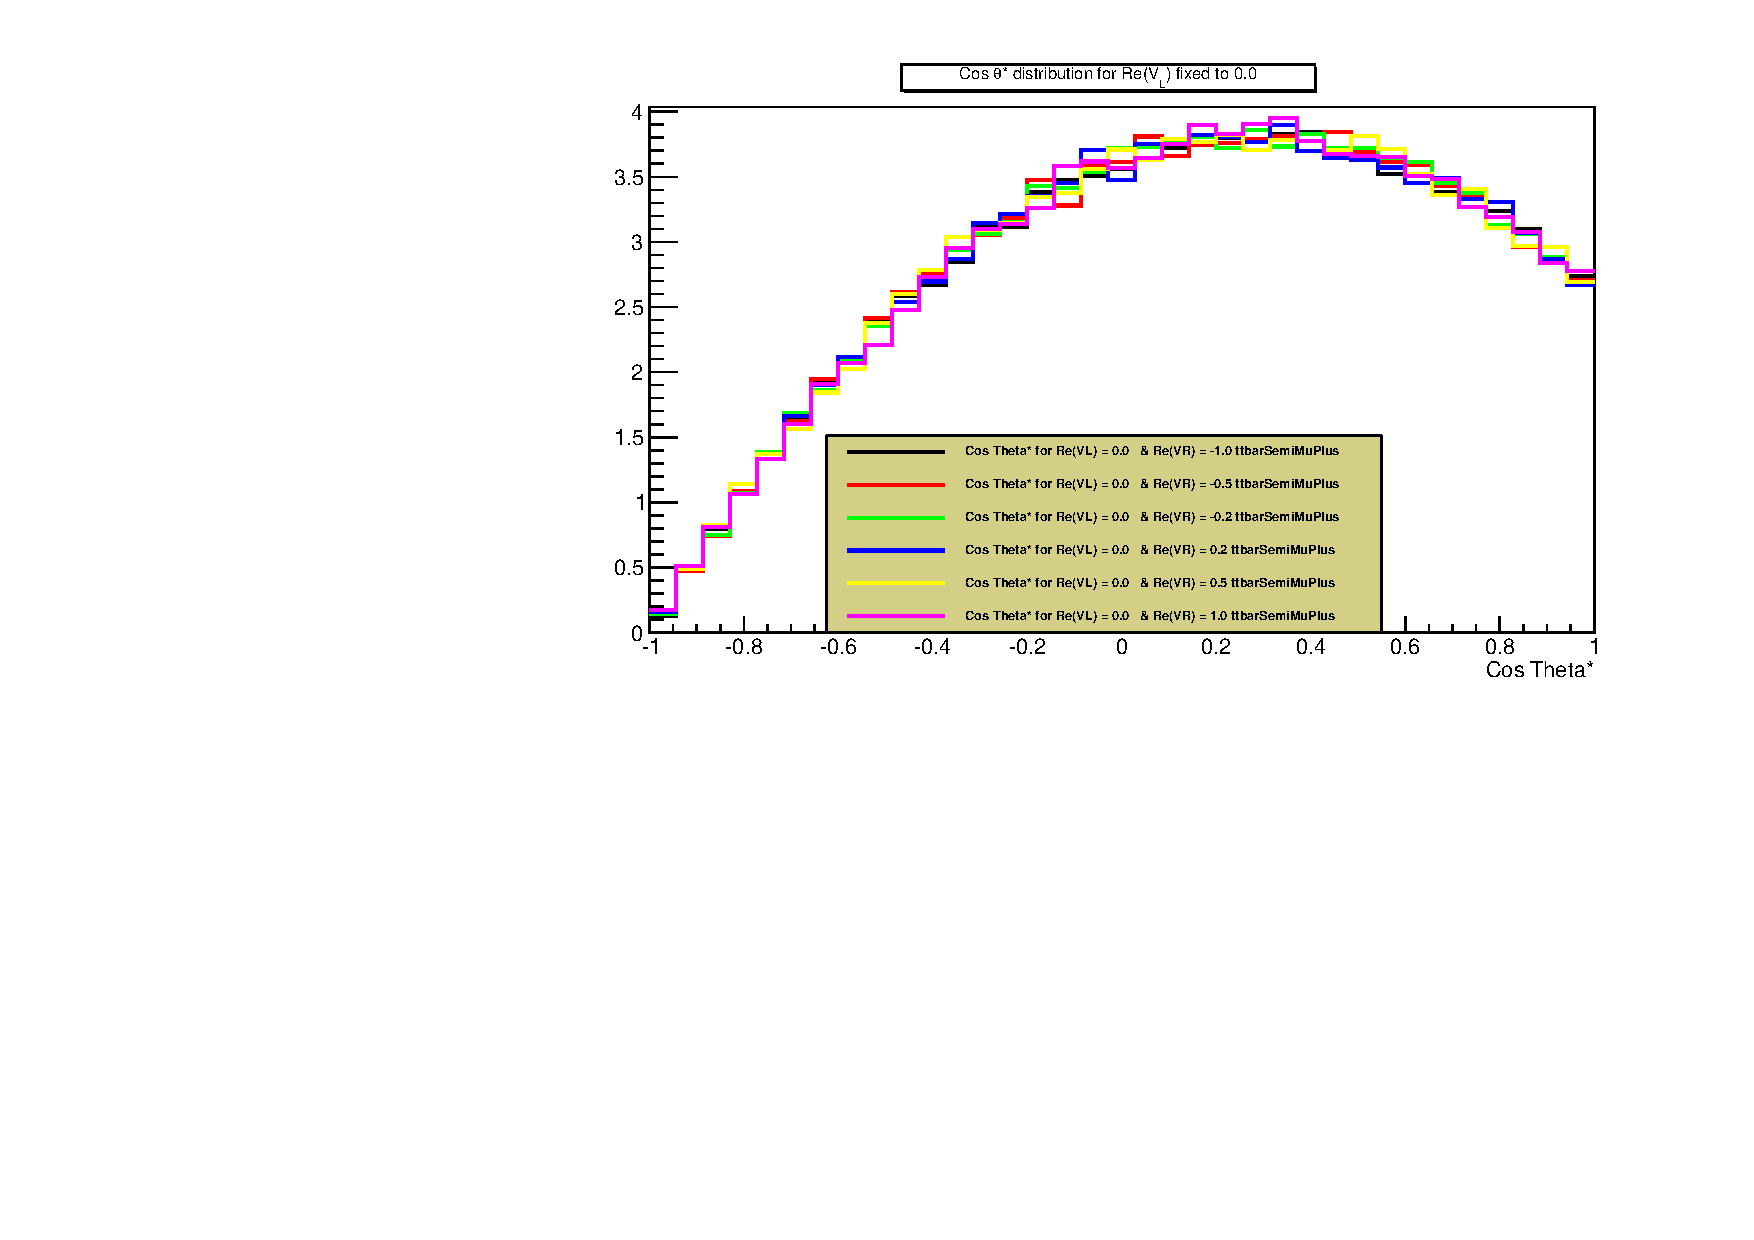
\includegraphics[width = 0.45 \textwidth]{Afbeeldingen/Chapter_LinkWithTopWidth/CosThetaResults/RVLvsRVR/RVLRVR_CosTheta_RVLFixedTo00.pdf}\\  %RVR varied
 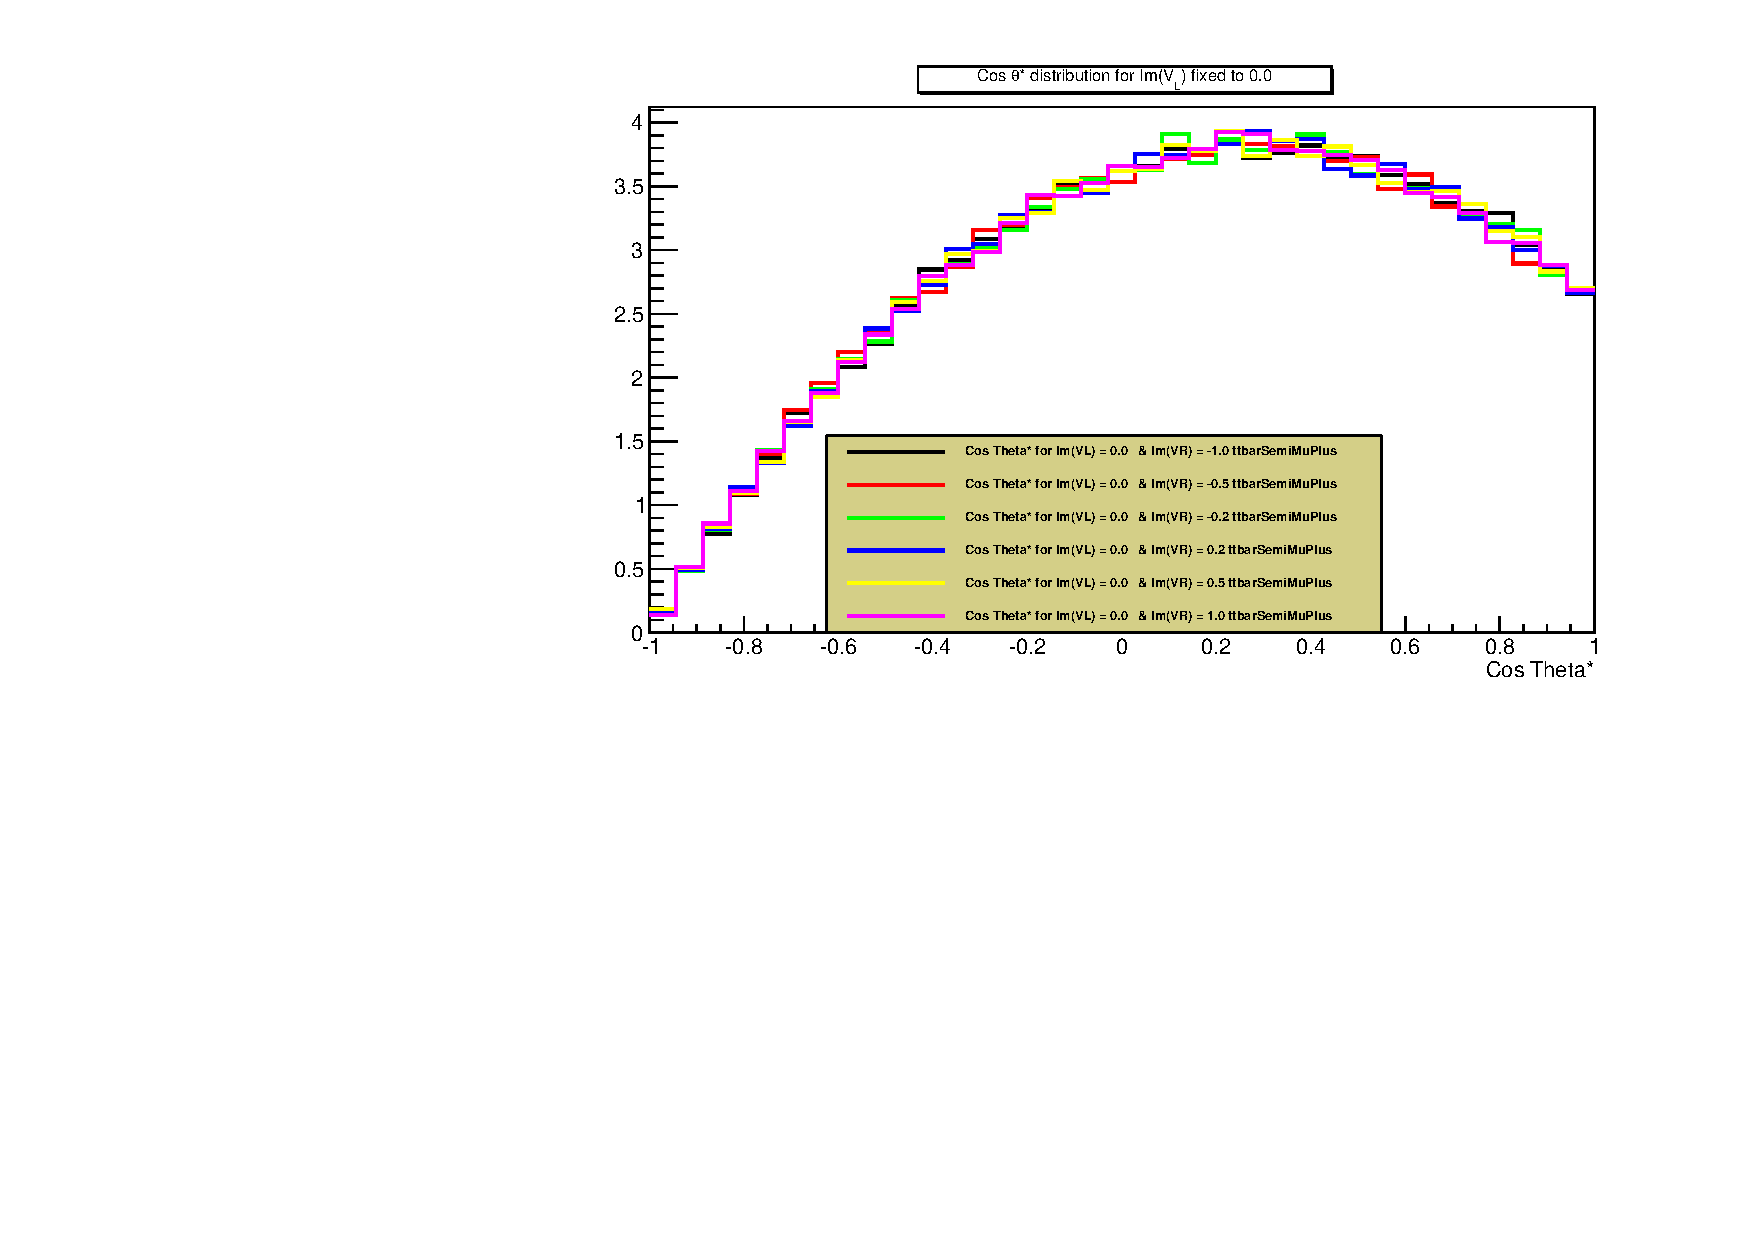
\includegraphics[width = 0.45 \textwidth]{Afbeeldingen/Chapter_LinkWithTopWidth/CosThetaResults/IVLvsIVR/IVLIVR_CosTheta_IVLFixedTo00.pdf}    %IVR varied
 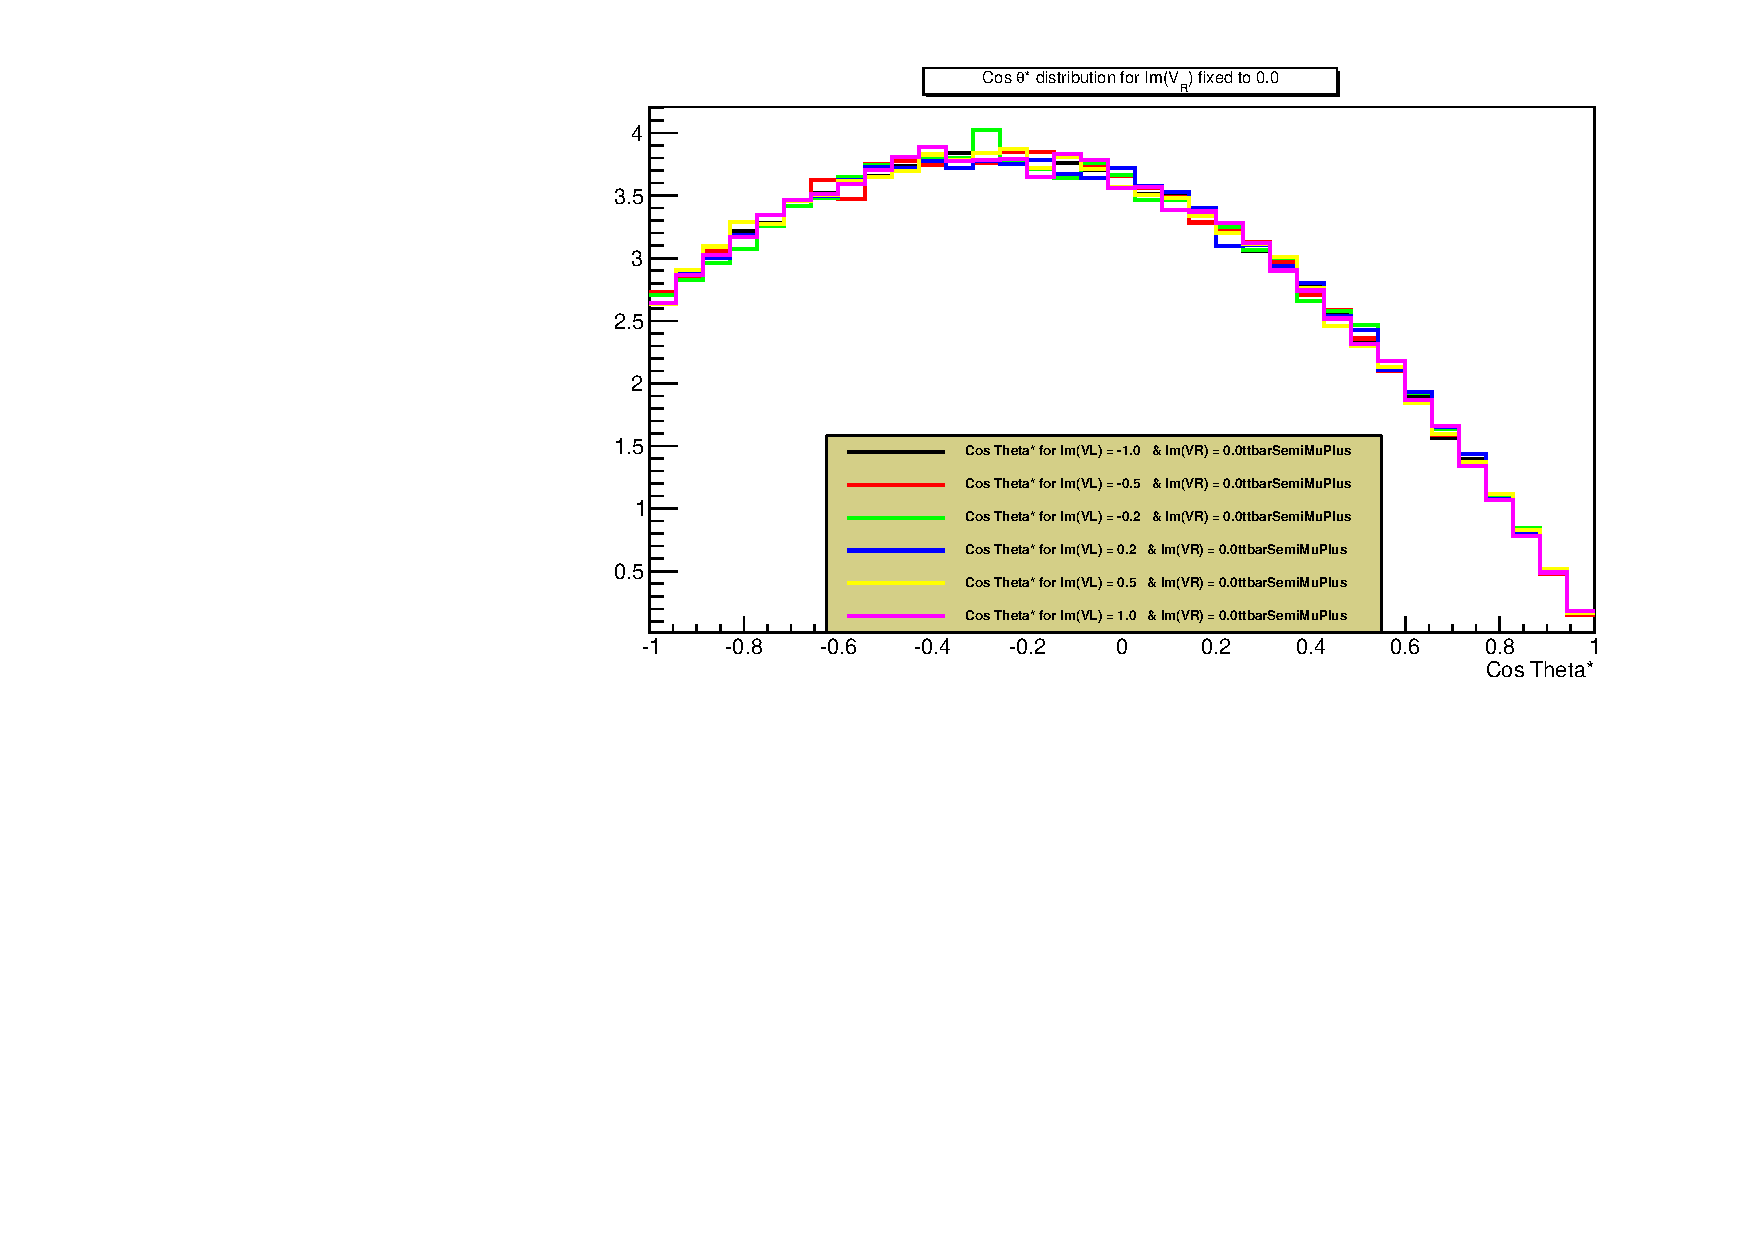
\includegraphics[width = 0.45 \textwidth]{Afbeeldingen/Chapter_LinkWithTopWidth/CosThetaResults/IVLvsIVR/IVLIVR_CosTheta_IVRFixedTo00.pdf}\\  %IVL varied
 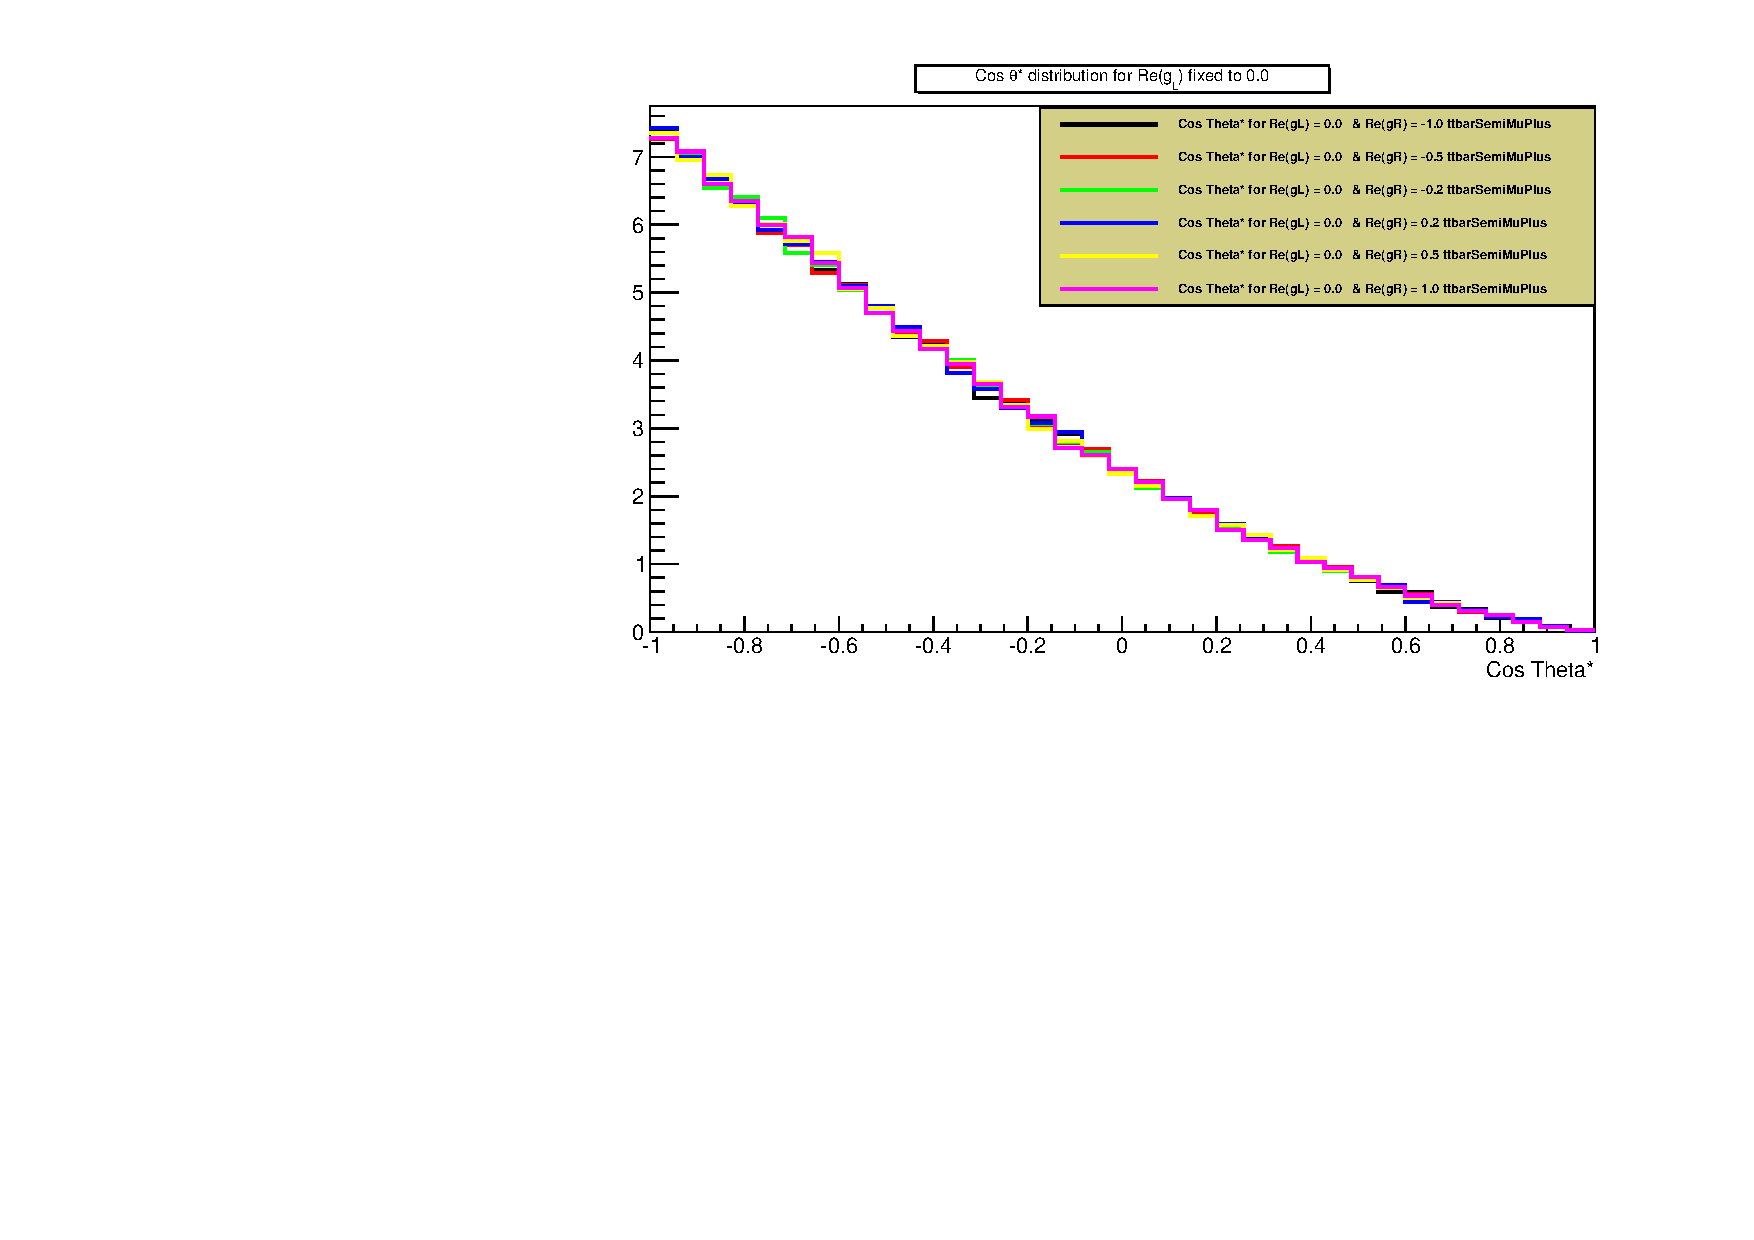
\includegraphics[width = 0.45 \textwidth]{Afbeeldingen/Chapter_LinkWithTopWidth/CosThetaResults/RgRvsRgL/RgLRgR_CosTheta_RgLFixedTo00.pdf}    %RgR varied
 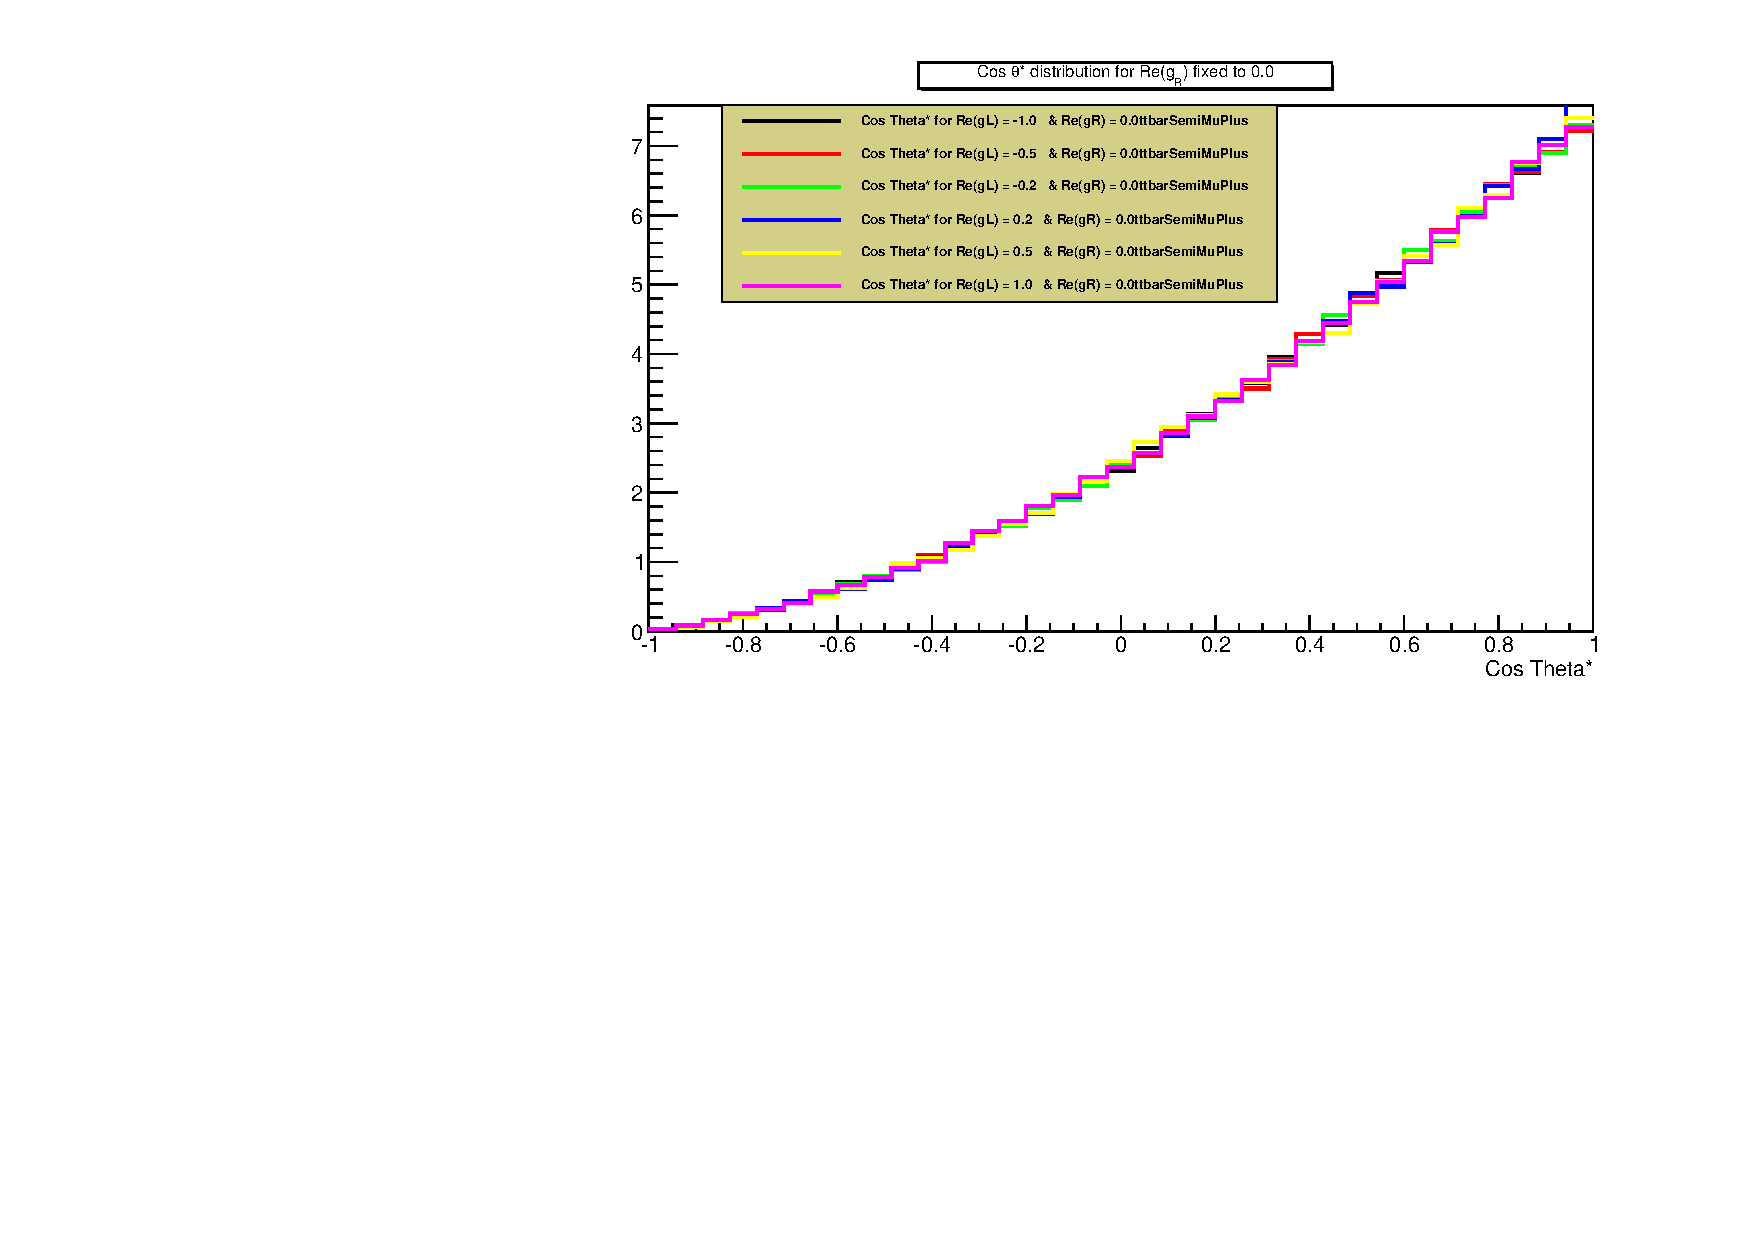
\includegraphics[width = 0.45 \textwidth]{Afbeeldingen/Chapter_LinkWithTopWidth/CosThetaResults/RgRvsRgL/RgLRgR_CosTheta_RgRFixedTo00.pdf}    %RgL varied
 \caption{Distributions of \csTh for configurations where only one of the Wtb-coupling coefficients is non-zero while the other one is varied between $-1$ and $1$. The two upper distributions show the case when only the real part of the two vector couplings is non-zero while the two middle ones represent the case when only their imaginary part is non-zero. Finally the two lower distributions give the \csTh distribution for the real part of the tensor couplings. The same conclusion holds for all distributions shown here, namely that no shape difference occurs when only one of the couplings is non-zero as was indicated by the formulas given above.}
 \label{fig::CosThetaOneCoupling}
\end{figure}

It is important to note that the same is also true when only the real and imaginary part of one coupling are varied. In those cases there is also no interference between different coupling constants which is necessary in order to introduce a different between the partial widths and the total width. For example when considering only the left-handed vector coupling, the only term which remains in the width definitions is $\vert V_{L} \vert^{2}$ $=$ $Re(V_{L})^{2} + Im(V_{L})^{2}$. However since it does not matter whether this term consists of both the real and the imaginary part or only the real part, it will cancel out when dividing the partial width part by the total width. This behavior is indeed retrieved in the \csTh distributions, as can be seen in Figure \ref{fig::CosThetaOneFullCoupling}.\\

\begin{figure}[h!]
 \centering
 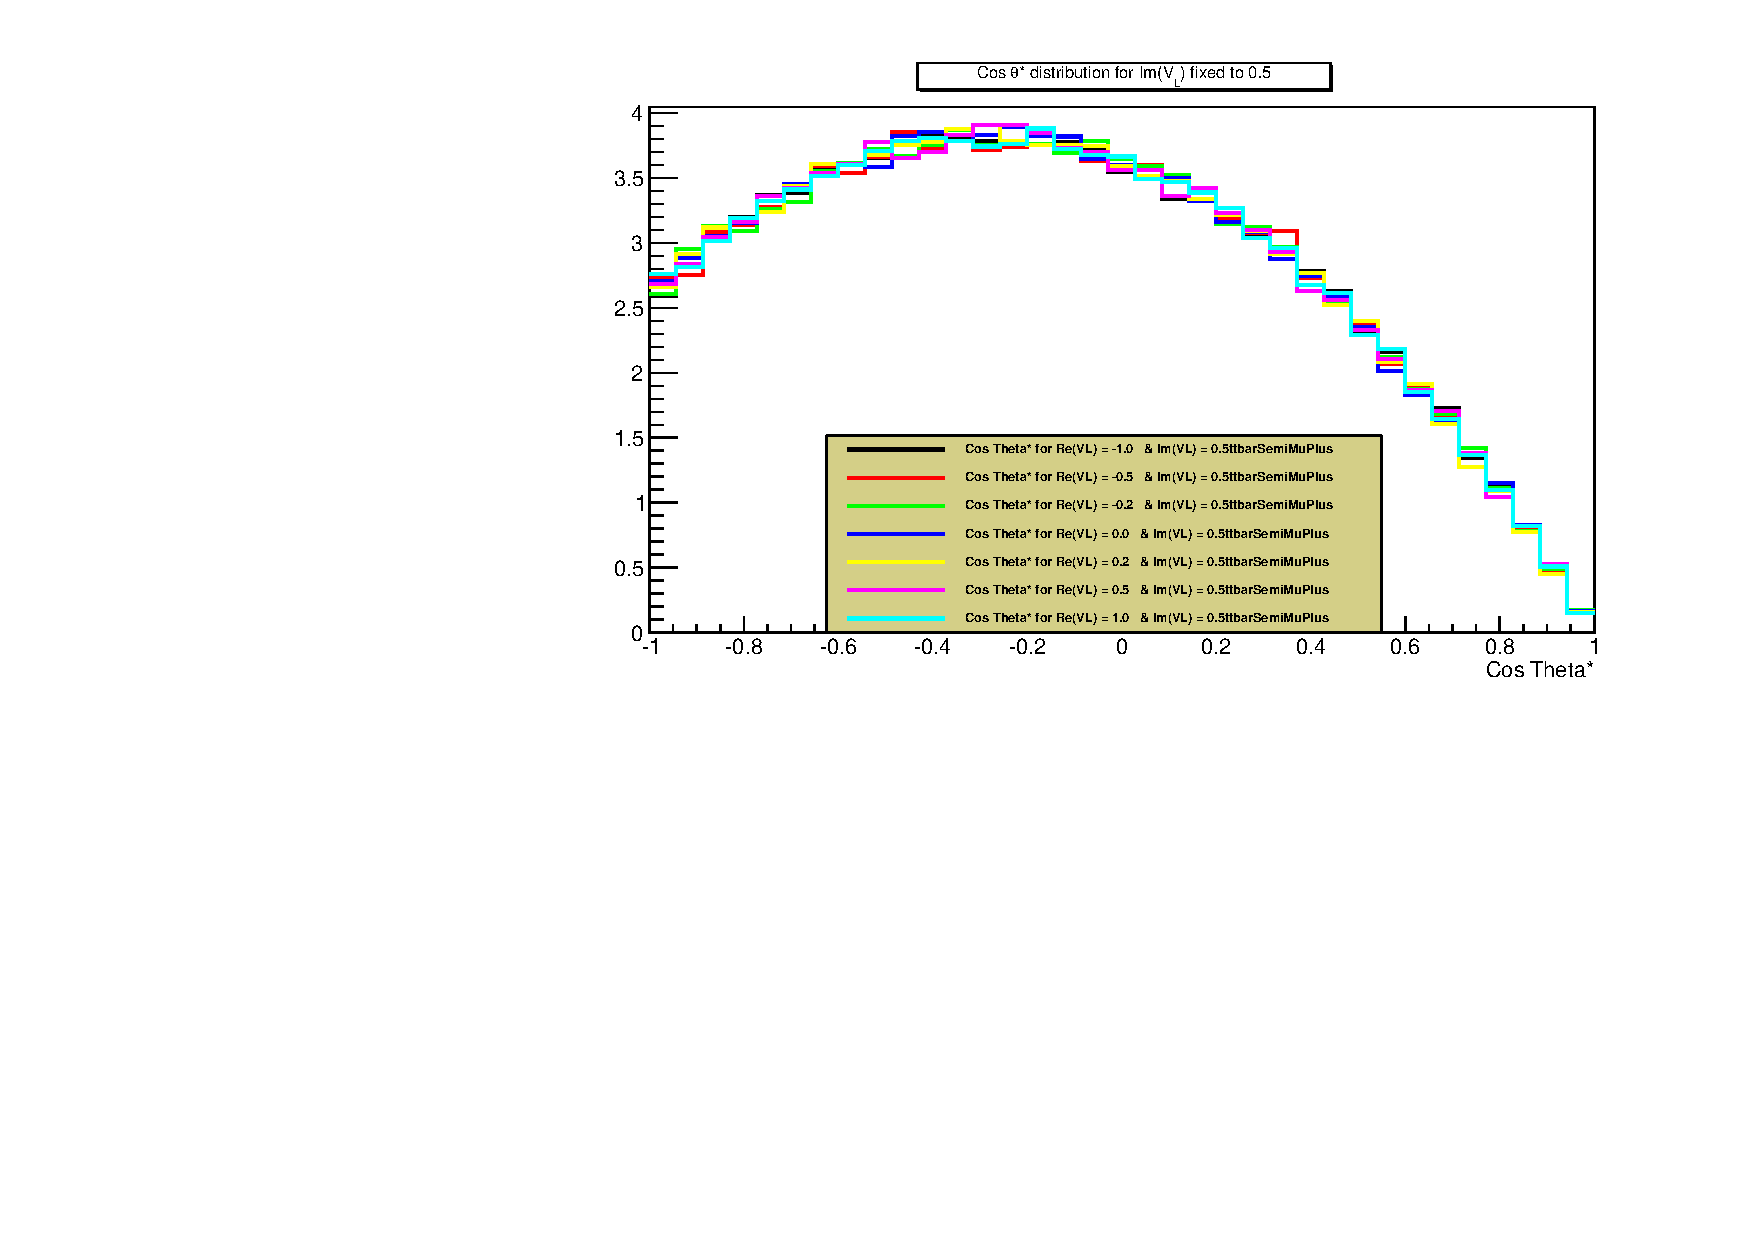
\includegraphics[width = 0.45 \textwidth]{Afbeeldingen/Chapter_LinkWithTopWidth/CosThetaResults/RVLvsIVL/RVLIVL_CosTheta_IVLFixedTo05.pdf}
 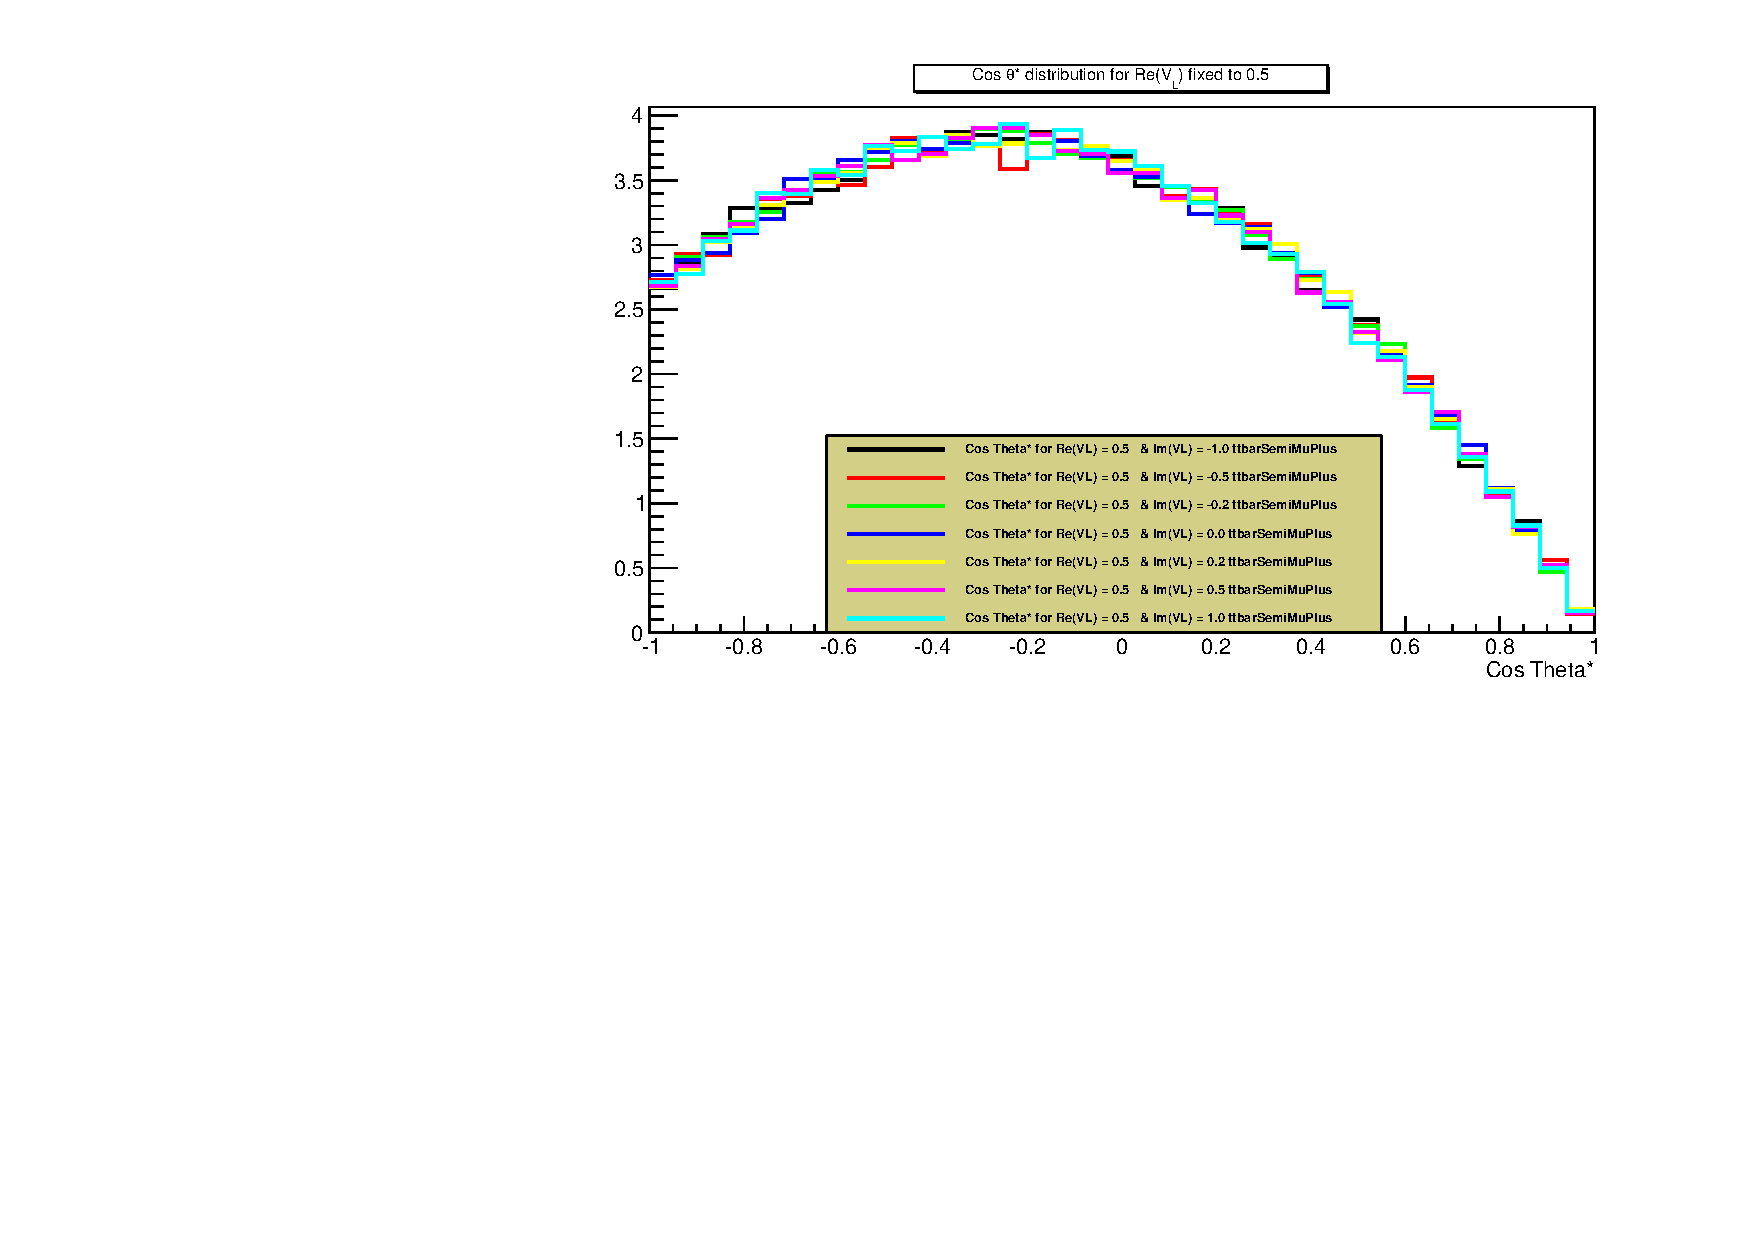
\includegraphics[width = 0.45 \textwidth]{Afbeeldingen/Chapter_LinkWithTopWidth/CosThetaResults/RVLvsIVL/RVLIVL_CosTheta_RVLFixedTo05.pdf}\\
 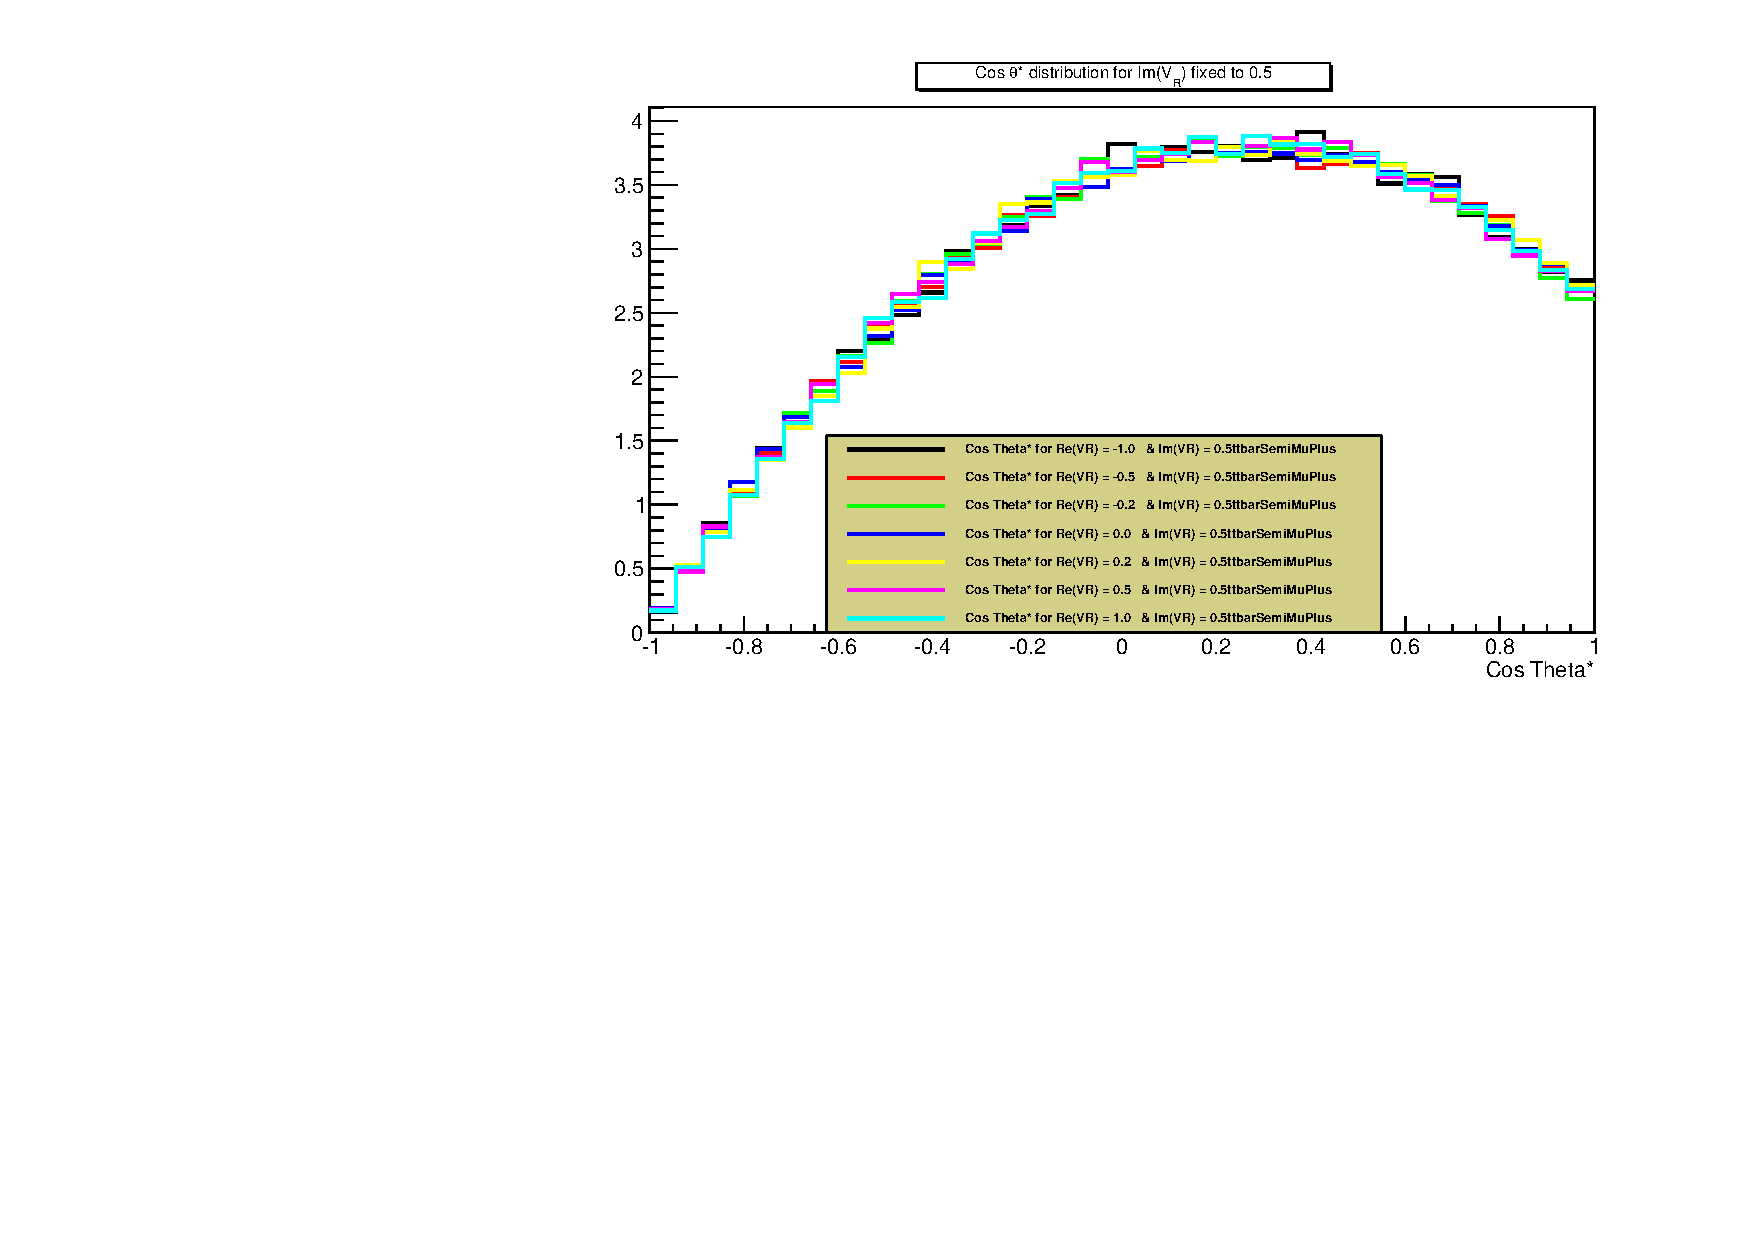
\includegraphics[width = 0.45 \textwidth]{Afbeeldingen/Chapter_LinkWithTopWidth/CosThetaResults/RVRvsIVR/RVRIVR_CosTheta_IVRFixedTo05.pdf}
 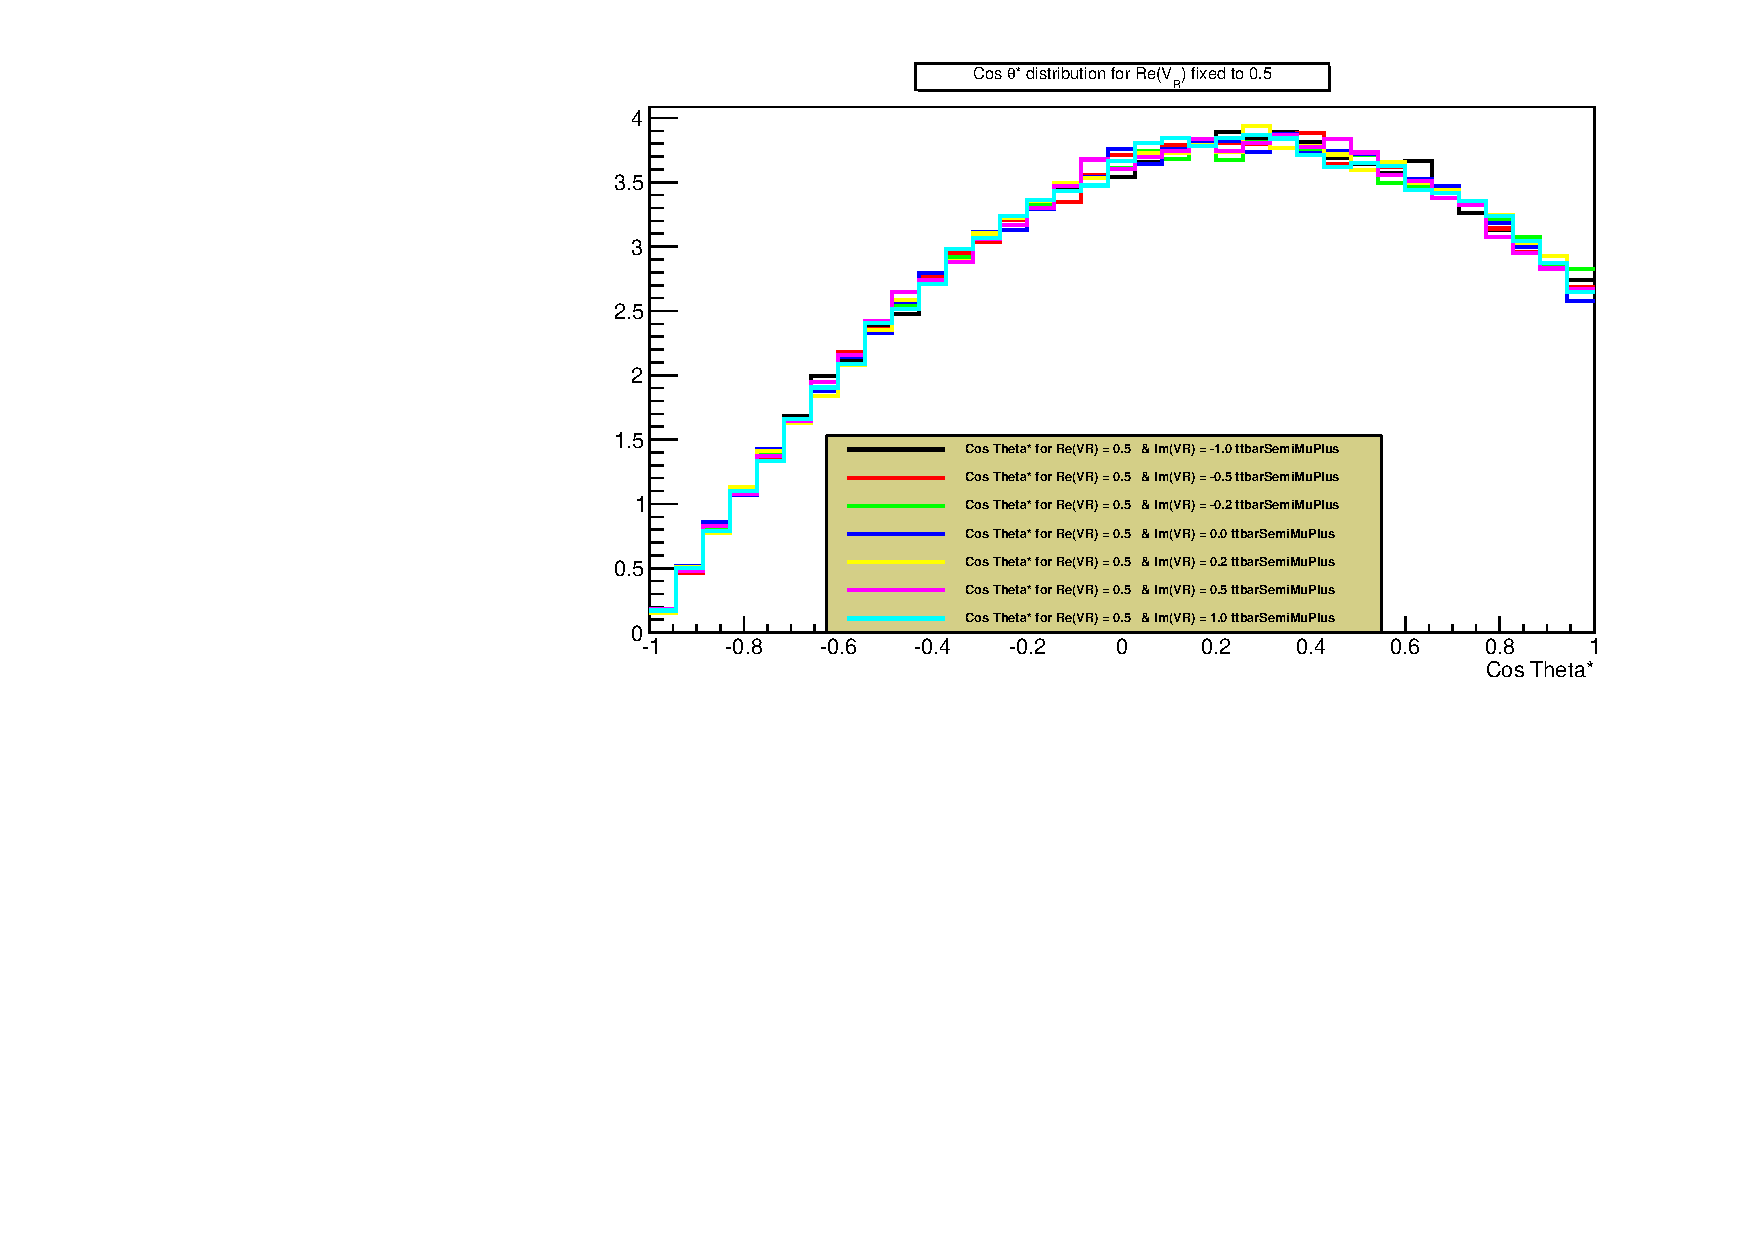
\includegraphics[width = 0.45 \textwidth]{Afbeeldingen/Chapter_LinkWithTopWidth/CosThetaResults/RVRvsIVR/RVRIVR_CosTheta_RVRFixedTo05.pdf}
 \caption{}
 \label{fig::CosThetaOneFullCoupling}
\end{figure}

\subsection{Massless b-limit}

Within the Wtb interaction the mass of the bottom quark is almost negligible compared to the massive W-boson and the top quark. Hence it is rather standard to use a so-called massless b-limit when considering the Wtb interaction, an approach which also explains the suppression of the right-handed helicity fraction of the W-boson.\\
When applying this assumption, the partial and total width formulas can be simplified significantly as will be shown in the following equations since the terms containing $x_{b}$ can be neglected. For simplicity only the real parts of the vector couplings are considered, but the same is true for other combinations.

\begin{eqnarray}
 \Gamma_{0}   & = & \frac{g^{2} \vert \vec{q}}{32 \pi} \frac{m_{t}^{2}}{m_{W}^{2}} \left[ \vert V_{L} \vert^{2} + \vert V_{R} \vert^{2} \right] (1 - x_{W}^{2} ) \\
 \Gamma_{R,L} & = & \frac{g^{2} \vert \vec{q}}{32 \pi} \frac{m_{t}^{2}}{m_{W}^{2}} \left[ \vert V_{L} \vert^{2} + \vert V_{R} \vert^{2} \right] (1 - x_{W}^{2})  \nonumber \\
              &   & \pm \frac{g^{2}}{64 \pi} \frac{m_{t}^{3}}{m_{W}^{2}} \left\lbrace -x_{W}^{2} \left[ \vert V_{L} \vert^{2} - \vert V_{R} \vert^{2}  \right] \right\rbrace (1-2x_{W}^{2} + x_{W}^{4})\\
 \Gamma       & = & \frac{g^{2} \vert \vec{q}}{32 \pi} \frac{m_{t}^{2}}{m_{W}^{2}} \left[ \vert V_{L} \vert^{2} + \vert V_{R} \vert^{2} \right] (1 + x_{W}^{2} - 2 x_{W}^{4})
\end{eqnarray}

From this can be seen that the longitudinal helicity fraction is not influenced at all when working in the massless b-limit. The right-handed and left-handed helicity fractions, on the other hand, have an opposite coupling-coefficient dependent part. This is again clearly visible in the studied \csTh distributions, which all behave simiar around \csTh = $0$. This is shown in Figure \ref{fig::CosThetaRVLRVR}.

\begin{figure}[h!]
 \centering
 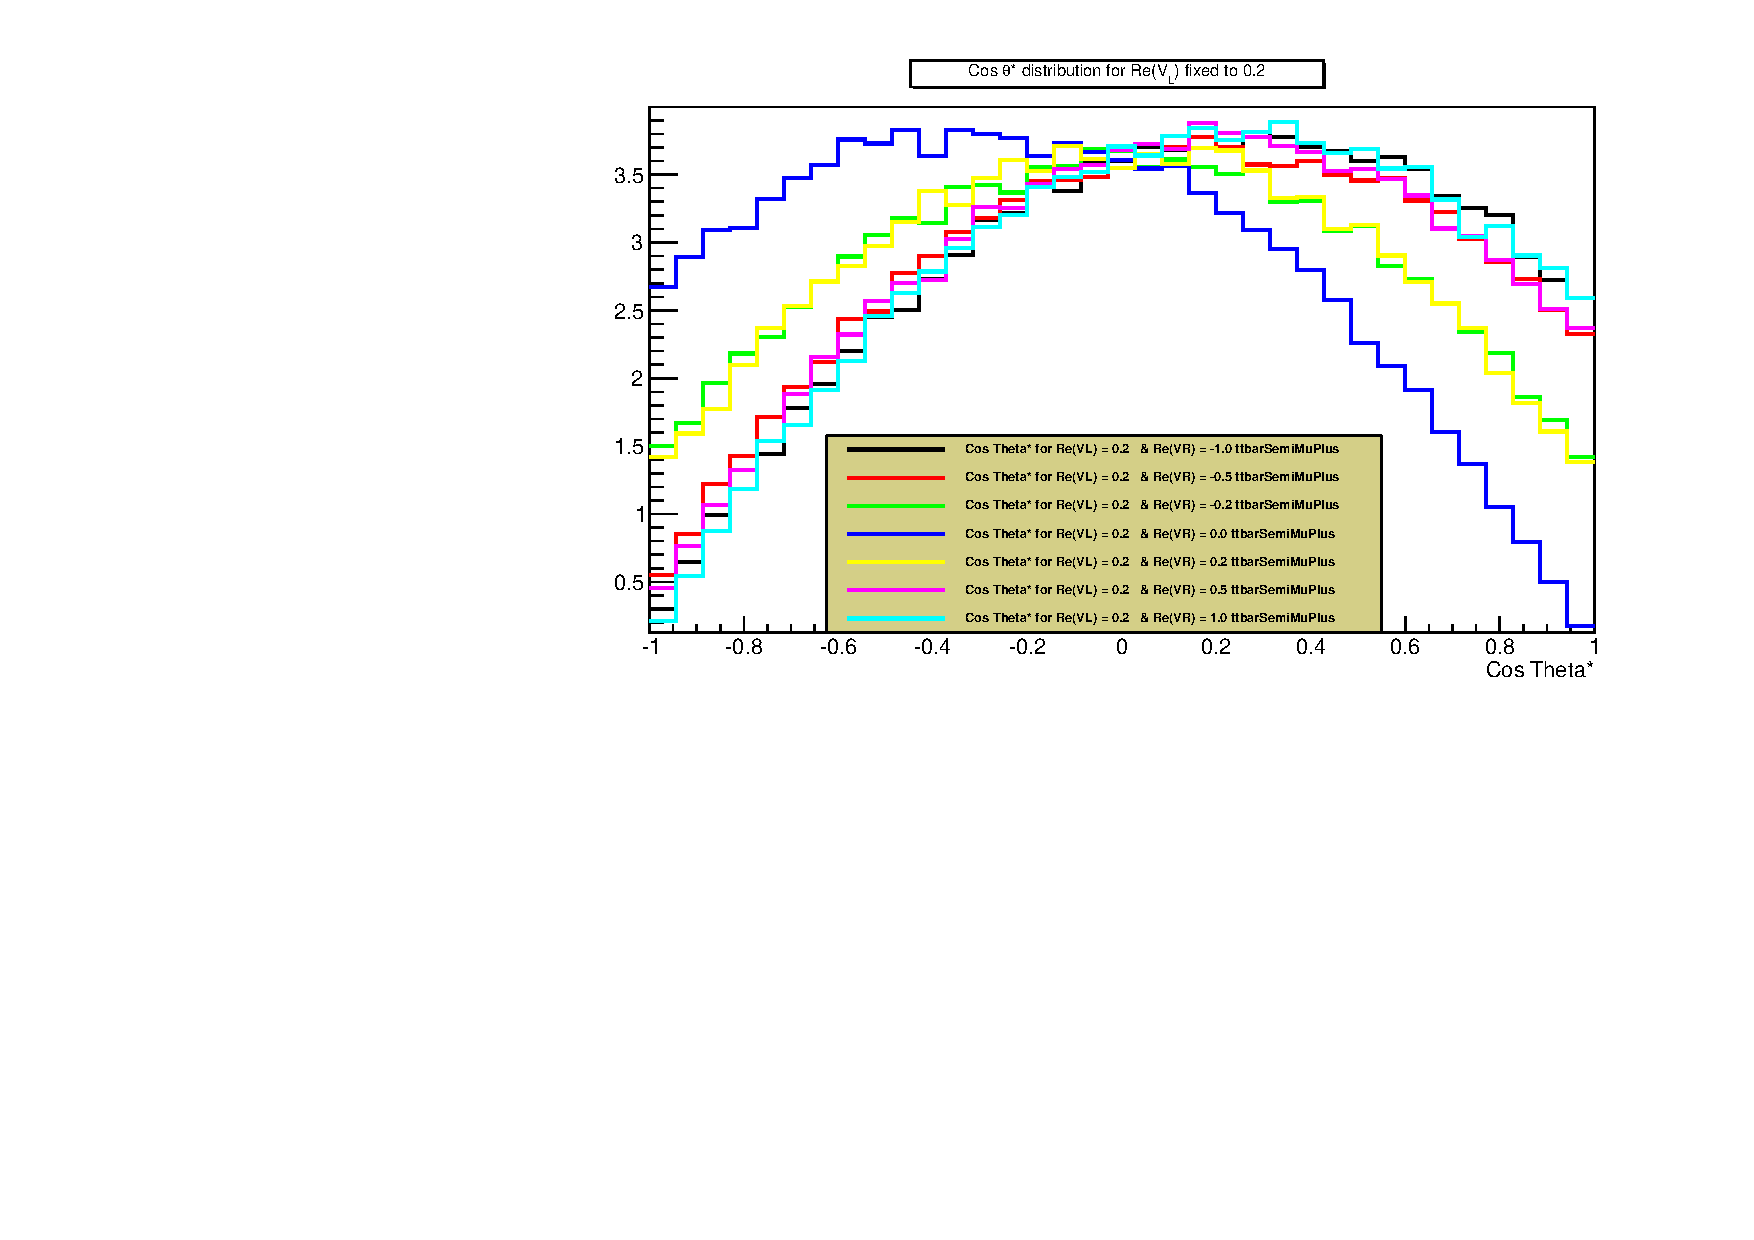
\includegraphics[width = 0.45 \textwidth]{Afbeeldingen/Chapter_LinkWithTopWidth/CosThetaResults/RVLvsRVR/RVLRVR_CosTheta_RVLFixedTo02.pdf}
 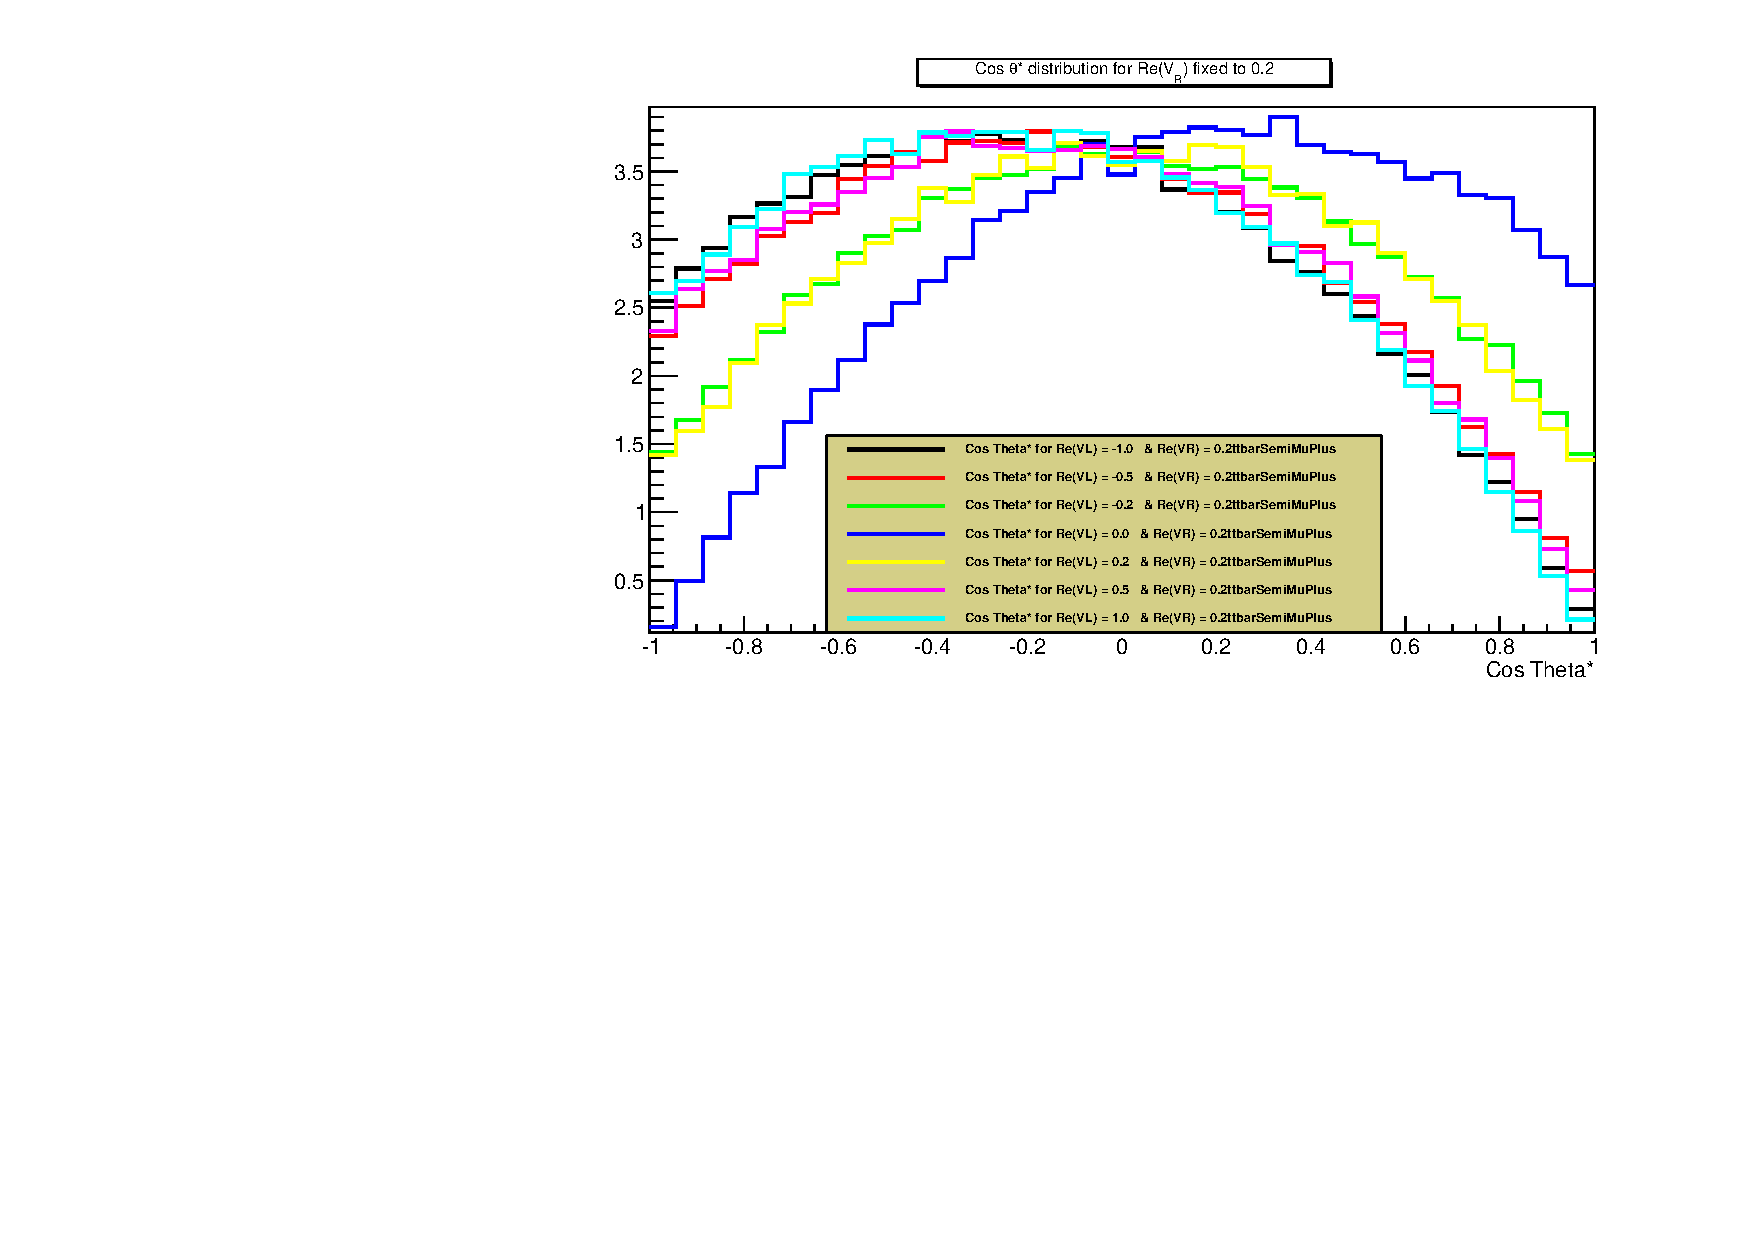
\includegraphics[width = 0.45 \textwidth]{Afbeeldingen/Chapter_LinkWithTopWidth/CosThetaResults/RVLvsRVR/RVLRVR_CosTheta_RVRFixedTo02.pdf}
 \caption{...}
 \label{fig::CosThetaRVLRVR}
\end{figure}

\subsection{Only 1 coupling non-zero within the massless b-limit}

The equations defined when considering only 1 non-zero coupling, Equations (\ref{eq::F0MasslessB}) and (\ref{eq::FRLMasslessB}), can be simplified even further when assuming the massless b-limit.

\begin{eqnarray}
 F_{0}   & = & \frac{(1 - x_{W}^{2} - 2x_{b}^{2} -x_{W}^{2} x_{b}^{2} + x_{b}^{4})}{(1 + x_{W}^{2} - 2x_{b}^{2} - 2 x_{W}^{4} + x_{W}^{2} x_{b}^{2})} \\
 F_{R,L} & = & \frac{m_{W}^{2}}{m_{t}^{2}} \frac{(1 - x_{W}^{2} + x_{b}^{2})}{(1 + x_{W}^{2} - 2x_{b}^{2} - 2 x_{W}^{4} + x_{W}^{2} x_{b}^{2})} \nonumber \\
         &                                 & \pm \frac{m_{t}}{2 \vert \vec{q} \vert} \frac{ -x_{W}^{2} (1-x_{b}^{2})}{(1 + x_{W}^{2} - 2x_{b}^{2} - 2 x_{W}^{4} + x_{W}^{2} x_{b}^{2})} \label{eq::FRLMasslessB}
\end{eqnarray}

For the simplified case where only 1 of the couplings is varied the dependency on the top quark mass can be calculated explicitely by using Equations (\ref{eq::Simplified}). Applying these definitions changes Equations (\ref{eq::F0MasslessB}) and (\ref{eq::FRLMasslessB}) as follows\footnote{This because within this massless b-limit $\vert \vec{q} \vert$ can be simplified to $\frac{m_{t}^{2} - m_{W}^{2}}{2m_{t}}$.}:

\begin{subequations}
 \begin{align*}
  F_{0} & = \frac{1 - x_{W}^{2} - 2x_{b}^{2} -x_{W}^{2} x_{b}^{2} + x_{b}^{4}}{1 + x_{W}^{2} - 2x_{b}^{2} - 2 x_{W}^{4} + x_{W}^{2} x_{b}^{2}} \\
        & = \frac{1 - \frac{m_{W}^{2}}{m_{t}^{2}} - 2 \frac{m_{b}^{2}}{m_{t}^{2}} - \frac{m_{W}^{2}}{m_{t}^{2}} \frac{m_{b}^{2}}{m_{t}^{2}} + \frac{m_{b}^{4}}{m_{t}^{4}}}{1 + \frac{m_{W}^{2}}{m_{t}^{2}} - 2 \frac{m_{b}^{2}}{m_{t}^{2}} - 2 \frac{m_{W}^{4}}{m_{t}^{2}} + \frac{m_{W}^{2}}{m_{t}^{2}} \frac{m_{b}^{2}}{m_{t}^{2}}} \\
        & = \frac{m_{t}^{4}}{m_{t}^{4}} \frac{m_{t}^{4} - m_{W}^{2} m_{t}^{2} - 2m_{b}^{2} m_{t}^{2} - m_{W}^{2} m_{b}^{2} + m_{b}^{4}}{1 + m_{W}^{2} m_{t}^{2} - 2 m_{b}^{2} m_{t}^{2} - 2 m_{W}^{4} + m_{W}^{2} m_{b}^{2} + m_{b}^{4}} \\
        & \textcolor{green}{\approx_{m_{b} = 0}} \frac{m_{t}^{4} - m_{W}^{2} m_{t}^{2}}{m_{t}^{4} + m_{W}^{2} m_{t}^{2} - 2m_{W}^{4}}
 \end{align*}
\end{subequations}

\begin{subequations}
 \begin{align*}
  F_{R,L} = & ~\frac{m_{W}^{2}}{m_{t}^{2}} \frac{1 - x_{W}^{2} + x_{b}^{2}}{1 + x_{W}^{2} - 2x_{b}^{2} - 2 x_{W}^{4} + x_{W}^{2} x_{b}^{2}} \pm \frac{m_{t}}{2 \vert \vec{q} \vert} \frac{ -x_{W}^{2} (1-2x_{W}^{2} - 2x_{b}^{2} + x_{W}^{4} - 2x_{W}^{2} x_{b}^{2} + x_{b}^{4})}{1 + x_{W}^{2} - 2x_{b}^{2} - 2 x_{W}^{4} + x_{W}^{2} x_{b}^{2}} \\
          = & ~\frac{m_{t}^{4}}{m_{t}^{4}} \left\lbrace \frac{m_{W}^{2}}{m_{t}^{2}}  \frac{1 - m_{W}^{2}m_{t}^{2} + m_{b}^{2}m_{t}^{2}}{1 + m_{W}^{2}m_{t}^{2} - 2m_{b}^{2}m_{t}^{2} - 2 m_{W}^{4} + m_{W}^{2} m_{b}^{2}} \right. \\
            & ~\left. \pm \frac{m_{t}}{2 \vert \vec{q} \vert} \frac{ -m_{W}^{2}}{m_{t}^{2}} \frac{m_{t}^{4} - 2m_{W}^{2}m_{t}^{2} - 2m_{b}^{2}m_{t}^{2} + m_{W}^{4} - 2m_{W}^{2} m_{b}^{2} + m_{b}^{4}}{m_{t}^{4} + m_{W}^{2}m_{t}^{2} - 2m_{b}^{2}m_{t}^{2} - 2 m_{W}^{4} + m_{W}^{2} m_{b}^{2}} \right\rbrace \\          
          \textcolor{green}{\approx} & ~\frac{m_{W}^{2}}{m_{t}^{2}}  \frac{m_{t}^{4} - m_{W}^{2}m_{t}^{2}}{1 + m_{W}^{2}m_{t}^{2} - 2 m_{W}^{4}} \pm \frac{m_{t}}{2 \vert \vec{q} \vert} \frac{ -m_{W}^{2}}{m_{t}^{2}} \frac{m_{t}^{4} - 2m_{W}^{2}m_{t}^{2} + m_{W}^{4}}{m_{t}^{4} + m_{W}^{2}m_{t}^{2} - 2 m_{W}^{4}} \\
          \textcolor{green}{\approx} & ~\frac{m_{W}^{2}}{m_{t}^{2}}  \frac{m_{t}^{2}(m_{t}^{2} - m_{W}^{2})}{m_{t}^{4} + m_{W}^{2}m_{t}^{2} - 2 m_{W}^{4}} \pm \frac{2m_{t}^{2}}{2 (m_{t}^{2} - m_{W}^{2})} \frac{ -m_{W}^{2}}{m_{t}^{2}} \frac{(m_{t}^{2} - m_{W}^{2})^{2}}{m_{t}^{4} + m_{W}^{2}m_{t}^{2} - 2 m_{W}^{4}} \\
          \textcolor{green}{\approx} & ~m_{W}^{2} \left( \frac{m_{t}^{2} - m_{W}^{2}}{m_{t}^{4} + m_{W}^{2}m_{t}^{2} - 2 m_{W}^{4}} \right) \mp m_{W}^{2} \left( \frac{m_{t}^{2} - m_{W}^{2}}{m_{t}^{4} + m_{W}^{2}m_{t}^{2} - 2 m_{W}^{4}} \right) \\
          & = \left\{ \begin{array}{l} 
            ~ 0 \qquad \qquad \qquad \quad \quad ~~~ \textrm{for right-handed helicity fraction} \\
            ~2m_{W}^{2} \frac{m_{t}^{2} - m_{W}^{2}}{m_{t}^{4} + m_{W}^{2}m_{t}^{2} - 2 m_{W}^{4}} \quad \textrm{for left-handed helicity fraction}
          \end{array} \right. 
 \end{align*}
\end{subequations}

Hence when creating the \csTh distribution for different top-quark masses it is expected to see a clear shape diffence for the left-handed helicity fraction. As postulated by the Standard Model, no right-handed contribution is expected and from the above equation is clear that this contribution does not depend on the considered top-quark mass. Again this can be seen on the \csTh distributions when varying the top quark mass between $153$ GeV and $193$ GeV in steps of $10$ GeV, as shown in Figure \ref{fig::CosThetaTopMass}.

\begin{figure}[!h]
 \centering
 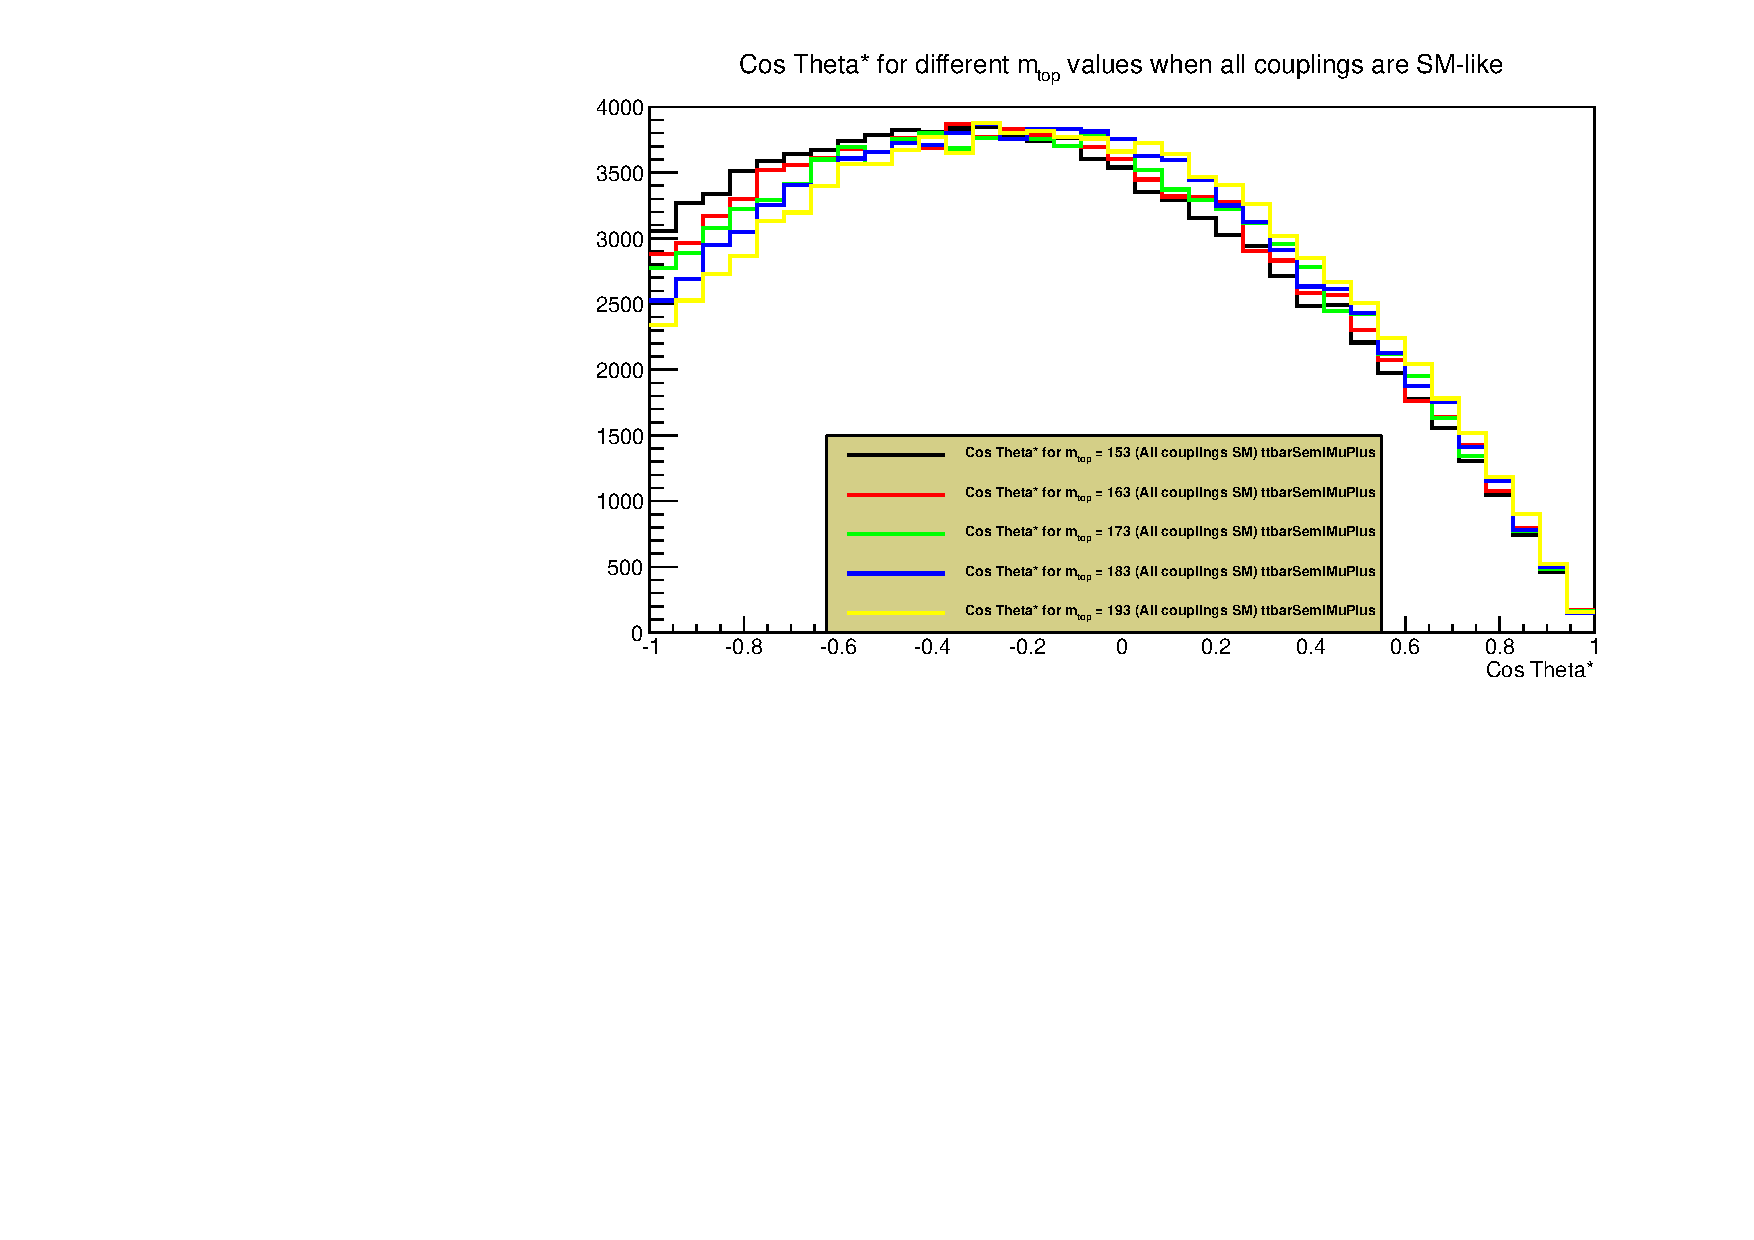
\includegraphics[width = 0.85 \textwidth]{Afbeeldingen/Chapter_LinkWithTopWidth/CosThetaResults/RVLvsRVR/RVLRVR_CosTheta_CosTheta_TopMassVaried.pdf}
 \caption{Distribution of \csTh when varying the top quark mass.}
 \label{fig::CosThetaTopMass}
\end{figure}

\section{Understanding symmetric behavior}

While studying all the different \csTh distributions for all the considered configurations, there was one peculiar observation. Every studied \csTh distribution clearly showed a symmetric relationship between the negative and positive part of each coupling coefficient. Again this can be explained using the partial top quark width definitions given above since with these equations it is possible to track down the term which depends on the sign of the coefficient.\\
The only terms which need to know the sign of the considered coefficient are the mixing terms such as $Re V_{L} V_{R}^{*}$ for example. However most of these mixing terms, and all of the most straightforward ones, are scaled with a factor $x_{b}$ implying that they are negligible in the massless b-limit. So mixing the vector and tensor couplings should give less symmetric \csTh distributions than the current studied mixings between vector and tensor couplings separately.\\
Figure \ref{fig::CosThetaHeavyB} clearly shows that the symmetric behavior is caused by low mass of the bottom quark. Both distributions represent an identical configuration, with the only difference the bottom-quark mass.

\begin{figure}[h!]
 \centering
 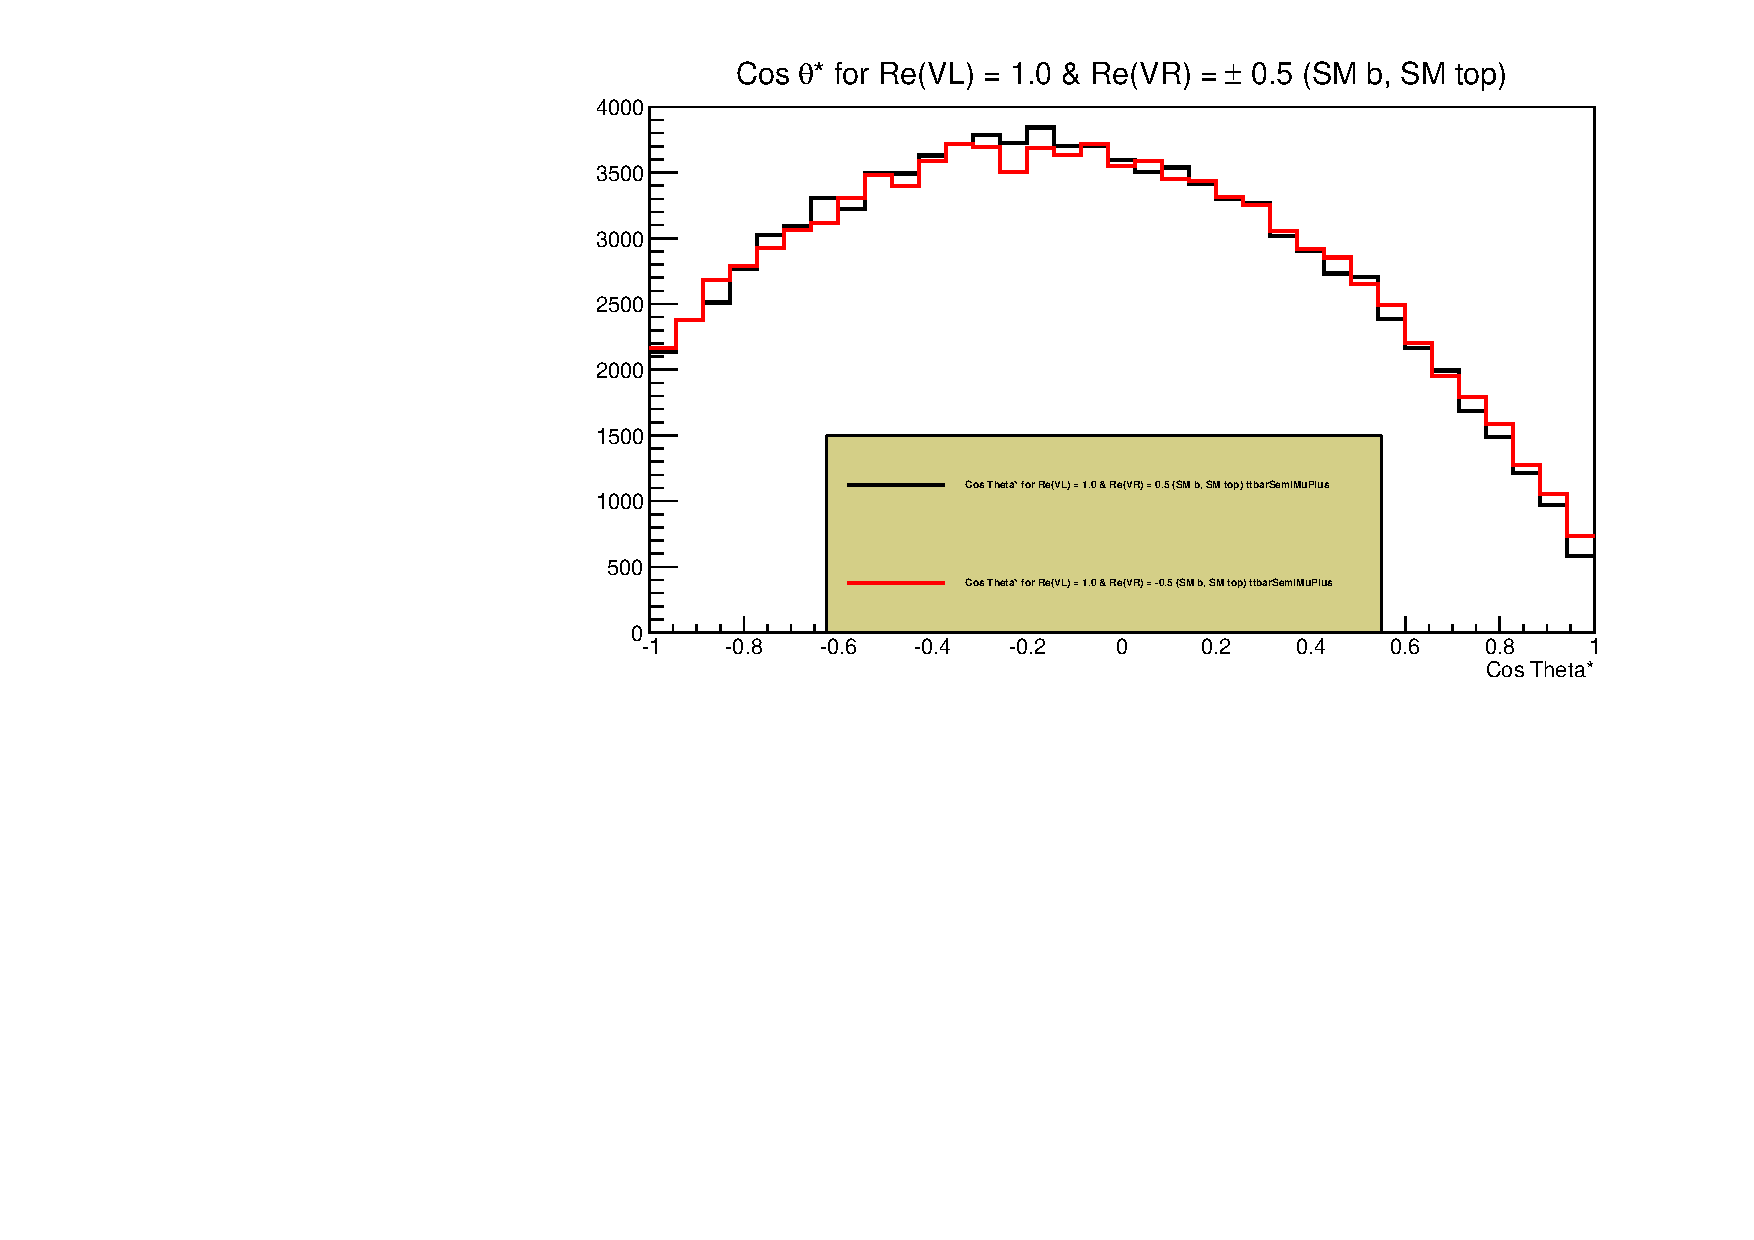
\includegraphics[width = 0.45 \textwidth]{Afbeeldingen/Chapter_LinkWithTopWidth/CosThetaResults/RVLvsRVR/RVLRVR_CosTheta_NormalBMass_RVRChange_RVLSM.pdf}
 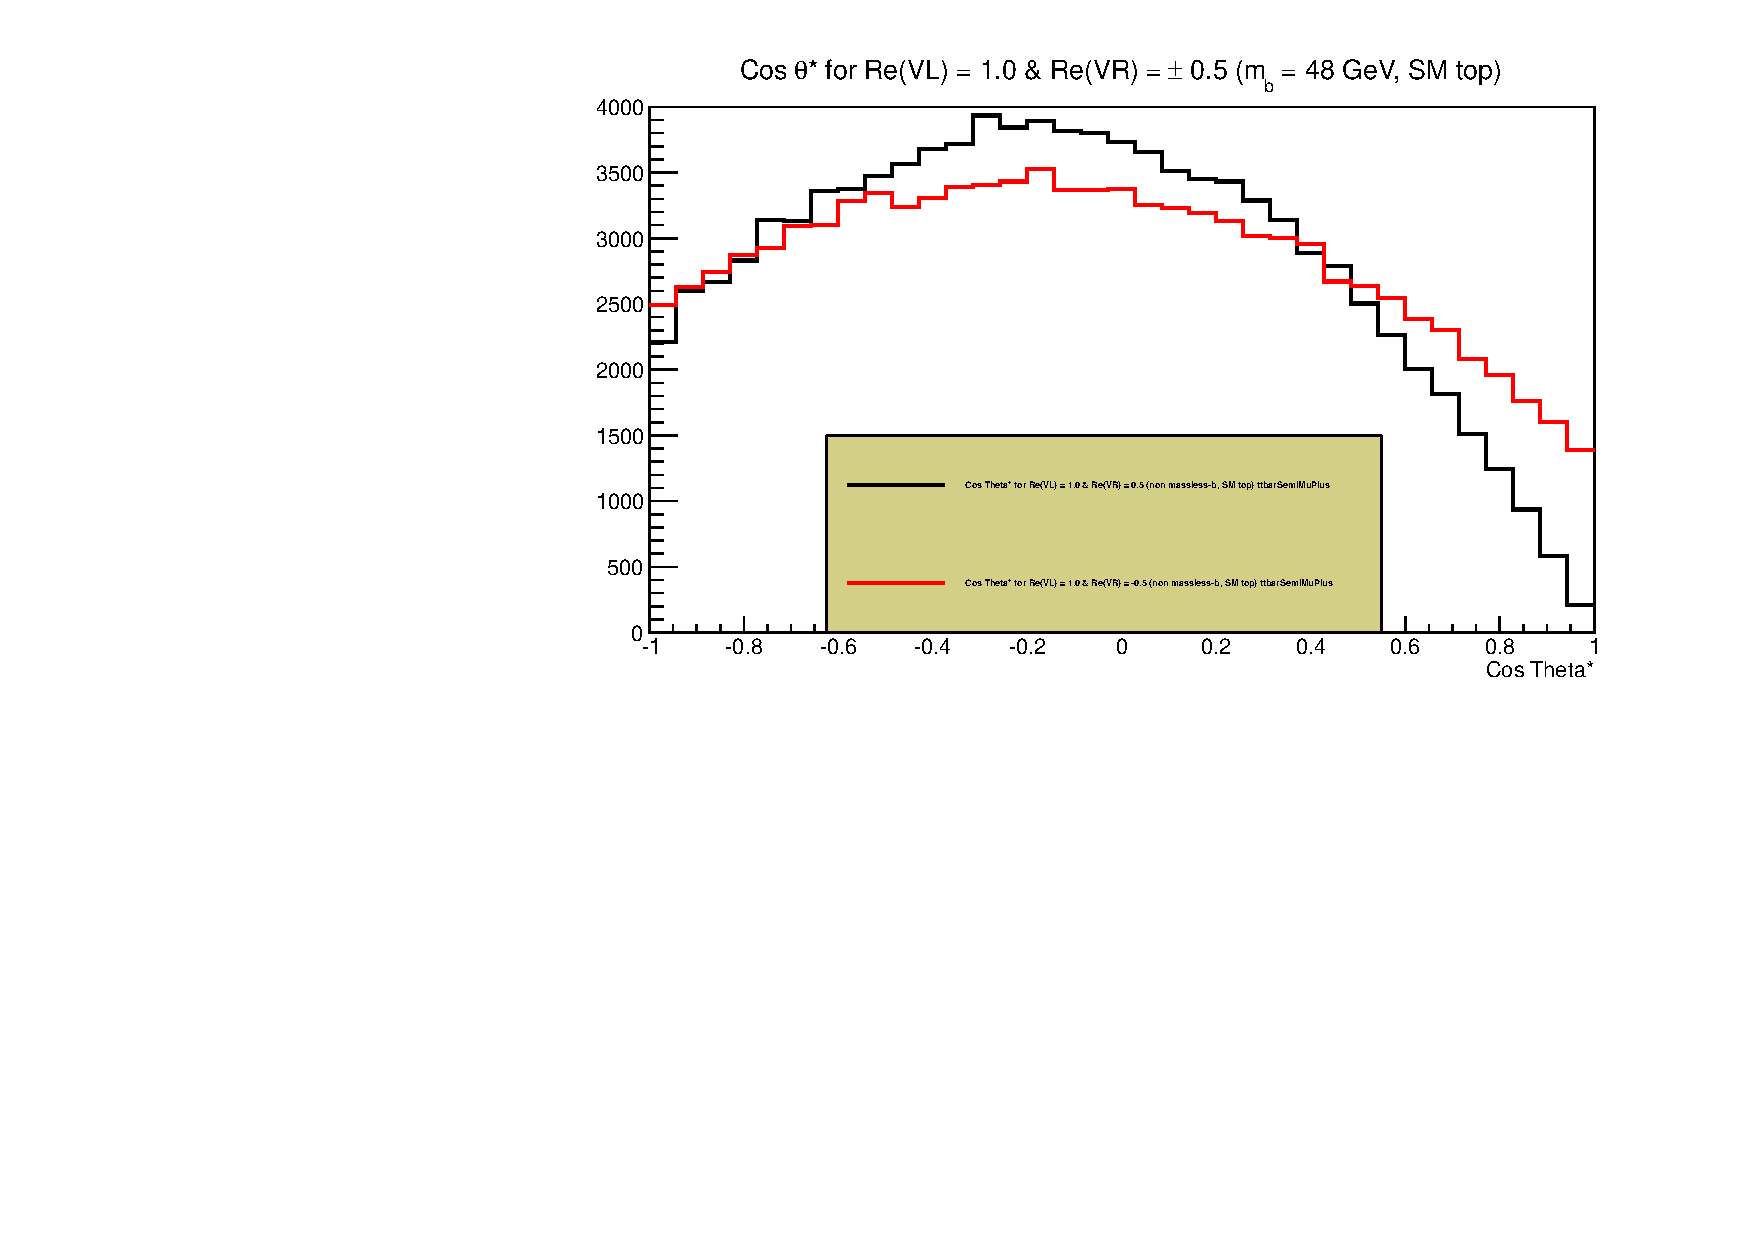
\includegraphics[width = 0.45 \textwidth]{Afbeeldingen/Chapter_LinkWithTopWidth/CosThetaResults/RVLvsRVR/RVLRVR_CosTheta_HeavyBMass_RVRChange_RVLSM.pdf}
 \caption{Influence of bottom-quark mass}
 \label{fig::CosThetaHeavyB}
\end{figure}